\documentclass{beamer}
\usepackage{xcolor}
\usepackage{natbib} % package to organize literature
\usepackage{booktabs}
\usepackage{graphicx} % to include graphics, gifs
\usepackage{lmodern} % to fix font size error, might be problematic with math symbols
\usepackage{tikz}
\usepackage{enumerate}
\usepackage{arydshln} % dashed lines
\usepackage{appendixnumberbeamer} % separate appendix numbering
\usepackage{fontawesome} % awesome icons
\usepackage[absolute,overlay]{textpos} % textbox in front of content

% Custom beamer settings
%\definecolor{beamer@sbred}{rgb}{0.65,0.15,0.18}
\definecolor{beamer@sbred}{rgb}{0.22,0.22,0.66}
\setbeamercolor{structure}{fg=beamer@sbred}
\setbeamertemplate{itemize items}[default]
\setbeamertemplate{enumerate items}[default]
\setbeamersize{text margin left=1em,text margin right=1em}
\setbeamercolor{frametitle}{fg=beamer@sbred}
\setbeamercolor{section in toc}{fg=beamer@sbred}
\setbeamercolor{subsection in toc}{fg=beamer@sbred!50}
\setbeamercolor*{block title example}{fg= white, bg= beamer@sbred!90}
\setbeamercolor*{block body example}{fg= black, bg= beamer@sbred!10}
\DeclareTextFontCommand{\emph}{\color{beamer@sbred}}

% link to table of contents
\makeatletter
\setbeamertemplate{footline}
{
    \leavevmode%
    \hbox{%
        \begin{beamercolorbox}[wd=.2\paperwidth,ht=2.25ex,dp=1ex,center]{}%
            \hyperlink{sec:main-content}{\emph{Content}} /  \hyperlink{sec:appendix-content}{\emph{Appendix}}
        \end{beamercolorbox}%
        \begin{beamercolorbox}[wd=.8\paperwidth,ht=2.25ex,dp=1ex,right]{date in head/foot}%
            %   \usebeamerfont{date in head/foot}\insertshortdate{}\hspace*{2em}
            \insertframenumber{} \hspace*{2ex}  / \hspace*{2ex} \inserttotalframenumber
            \hspace*{2ex} 
        \end{beamercolorbox}}%
        \vskip0pt%
    }
    \makeatother
\setbeamertemplate{navigation symbols}{}


\author{Patrick W. Kraft}
\title{Let's Talk Politics\\
{\large A Naive Approach for Measuring Political Sophistication}}
\institute{University of Barcelona}
\date{February 20\textsuperscript{th} 2020}
\titlegraphic{\vfill
\includegraphics[width=4cm]{fig/preferred.jpg}
%\hfill\includegraphics[width=3cm]{/data/Dropbox/Uni/Misc/Logos/logo.pdf}
}


\begin{document}
	
\frame{\titlepage}

\section*{Content}
\begin{frame}%[allowframebreaks]
\frametitle{Content}
\tableofcontents[hideallsubsections]
\end{frame}

\section{Theoretical Introduction}
% INTRODUCTION:
% Thank you very much, my name is Patrick Kraft and I am a PhD Candidate at the Department for Political Science at Stony Brook University. My research is located at the intersection of political behavior and methodology. In my dissertation, I analyze how citizens discuss their political beliefs in their own words. Verbally expressing your attitudes toward an issue is one of the most ubiquitous ways to engage in politics. Yet little research directly studies this basic feature of day-to-day political life. Building on recent advances in quantitative text analysis methods, I develop measures to systematically examine verbatim political attitude expression. A key argument in my thesis is that by analyzing how citizens describe their beliefs and discuss them with peers, we can make inferences about the nature of their attitudes. The research that I want to present today is one chapter out of my dissertations which focuses on political sophistication. I propose a new measure of political sophistication based on verbatim attitude expression in open-ended survey items.

%\begin{frame}{Introduction}
%\begin{itemize}
%\item Verbally \emph{expressing your attitudes} toward an issue is one of the most ubiquitous---yet rarely studied---ways to engage in politics.
%\item<2-> We can leverage how citizens talk about politics to make inferences about the \emph{nature of their attitudes}.
%\vspace{1em}
%\visible<3->{\begin{center}
%\emph{Words} do the work of \emph{politics}\\{\tiny\citep{graham2009liberals}}
%\end{center}}
%\vspace{1em}
%\item<4-> \emph{Research} program:
%\begin{enumerate}
%\item<5-> Study \emph{moralization} in political attitude expression
%\item \only<6-7>{Utilize open-ended responses to measure political \emph{sophistication}}\only<8>{\textbf{Utilize open-ended responses to measure political \emph{sophistication}}}
%\item<7-> Map \emph{social influence} processes in political \emph{discussions}
%\end{enumerate}
%\end{itemize}
%\end{frame}
%
%\begin{frame}{Overview}
%\tableofcontents[hideallsubsections]
%\end{frame}

\begin{frame}{Who scores higher on political knowledge?}
    \begin{center}
        \begin{tikzpicture}
            \node<1>[anchor=south west,inner sep=0] (image) at (0,0) {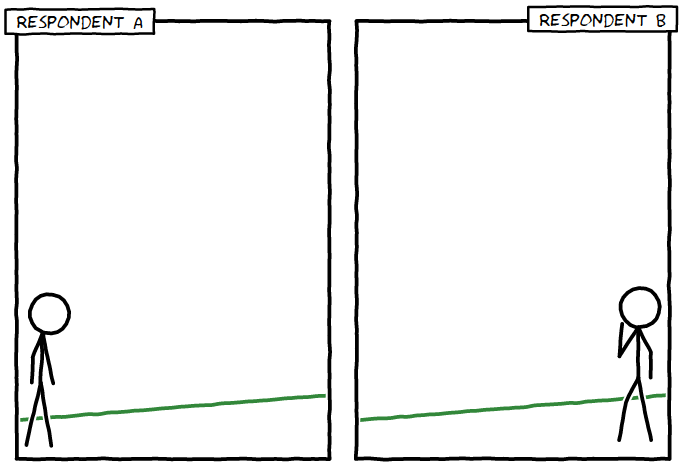
\includegraphics[width=.9\textwidth]{fig/Respondents0.png}};
            \node<2>[anchor=south west,inner sep=0] (image) at (0,0) {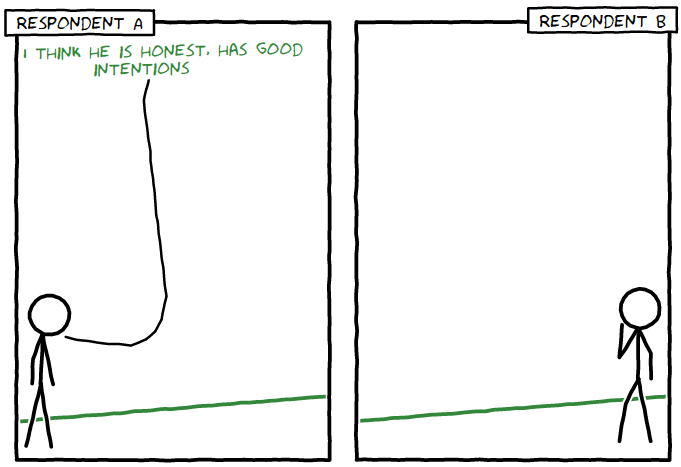
\includegraphics[width=.9\textwidth]{fig/Respondents1.png}};
            \node<3>[anchor=south west,inner sep=0] (image) at (0,0) {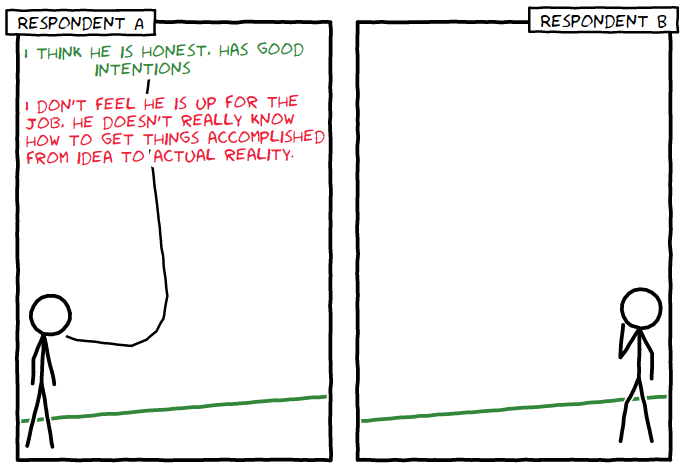
\includegraphics[width=.9\textwidth]{fig/Respondents2.png}};
            \node<4>[anchor=south west,inner sep=0] (image) at (0,0) {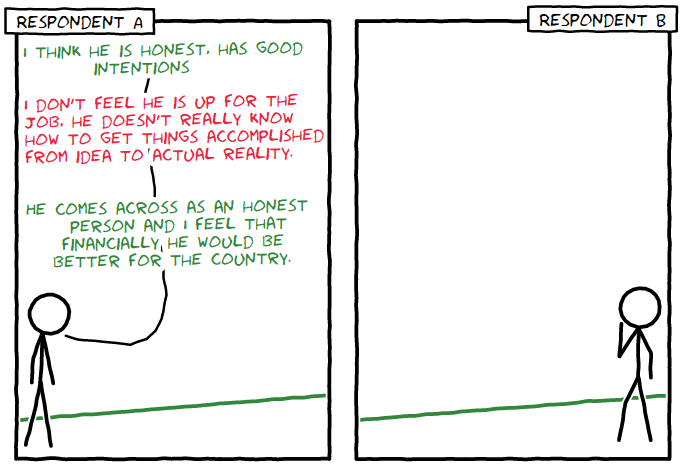
\includegraphics[width=.9\textwidth]{fig/Respondents3.png}};
            \node<5>[anchor=south west,inner sep=0] (image) at (0,0) {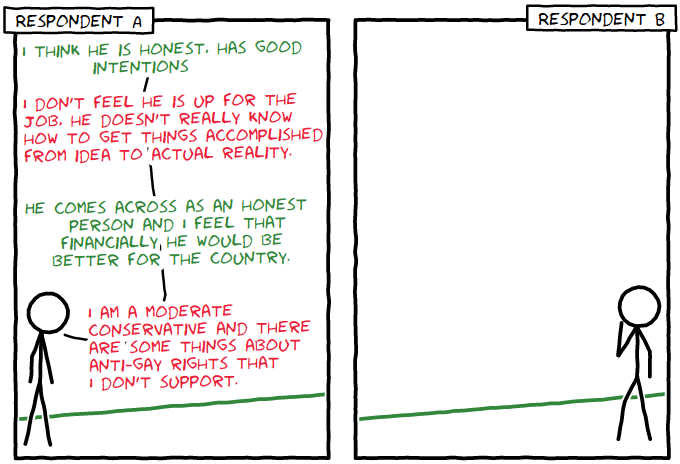
\includegraphics[width=.9\textwidth]{fig/Respondents4.png}};
            \node<6>[anchor=south west,inner sep=0] (image) at (0,0) {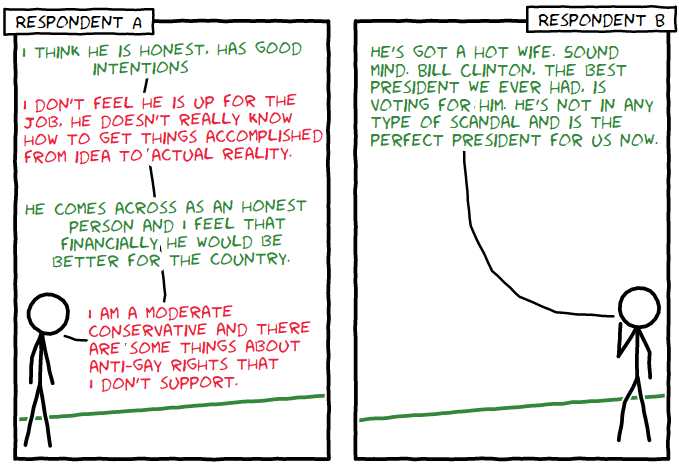
\includegraphics[width=.9\textwidth]{fig/Respondents5.png}};
            \node<7>[anchor=south west,inner sep=0] (image) at (0,0) {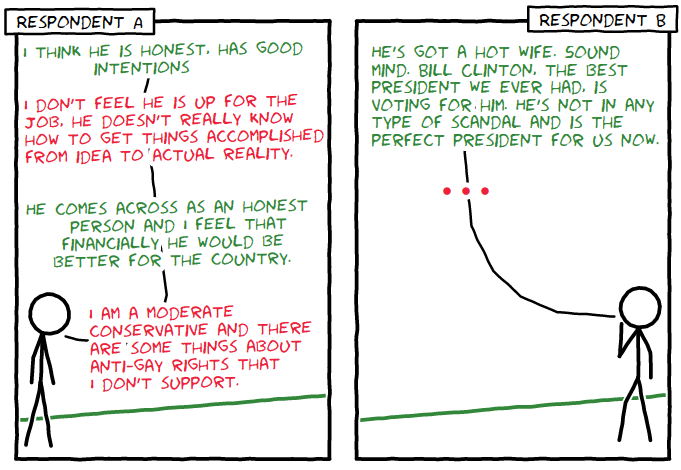
\includegraphics[width=.9\textwidth]{fig/Respondents6.png}};
            \node<8>[anchor=south west,inner sep=0] (image) at (0,0) {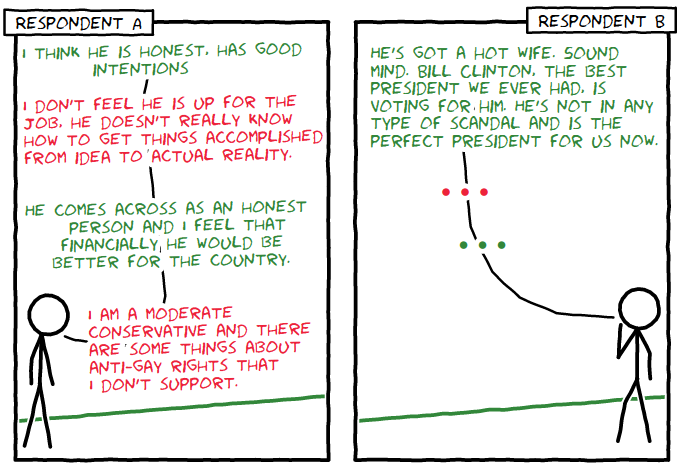
\includegraphics[width=.9\textwidth]{fig/Respondents7.png}};
            \node<9->[anchor=south west,inner sep=0] (image) at (0,0) {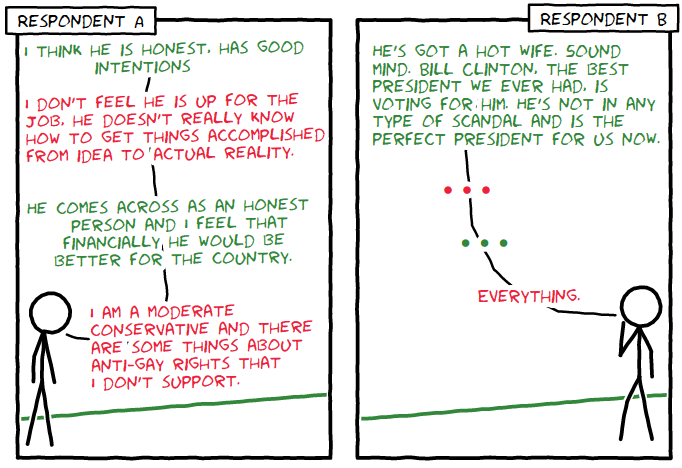
\includegraphics[width=.9\textwidth]{fig/Respondents8.png}};
            \node<10->[align=center,draw opacity=0,fill opacity=0.8,text opacity=1, white, fill=beamer@sbred] at (image.center) {\large Both respondents scored \\\Large\textbf{\color{red}{equally}}
            \\\large on the conventional political knowledge measure
            \\\large in the 2012 ANES!};
        \end{tikzpicture}
    \end{center}
\end{frame}

% OLD: I am interested in how individuals describe and justify their political attitudes, which can have important effects, especially in a social context. In my dissertation, I work a lot with open-ended responses.
% OLD: mention data source: ANES 2012, around 5000 respondents, online + f2f study
% I want to start with a little example. I am going to show you two sample responses to open-ended likes/dislikes items in the 2012 American National Election Study. Respondent A and B both described what they liked and disliked about the two major presidential candidates, Barack Obama and Mitt Romney. You know, back in the good old days when Presidential candidates were not considered completely crazy. Respondent A said the following:
% ... Respondent B, on the other hand, said...
% Now, who would you guess scored higher in factual political knowledge? Clearly, our intuition tells us that A seems more knowledgeable than B.

% However, it turns out that these two respondents scored equally on the conventional political knowledge measure in the 2012 ANES!
% factual knowledge: inquiring for example about the number of times an individual can be elected President of the United States, or how the current U.S. federal budget deficit compares to the deficit in the 1990s.

% In this talk, I basically want to convinvce you of two things:
% 1) there is meaningful variance in open-ended responses that is directly related to our conceptualization of political sophistication
% 2) we can gain new insights about the nature of sophistication if we utilize open-ended responses

% So how can we leverage this variation to measure political sophistication in attitude expression:
% Luskin: Sophistication is defined based on a belief system: (1) their \textsl{size} -- i.e. the number of cognitions, (2) their \textsl{range} -- i.e. the dispersion of cognition over categories, and (3) their \textsl{constraint} -- i.e. the extent to which cognitions are interconnected in a meaningful way.``

% How can we measure sophistication based on these open-ended responses? Well, the first possibility would be to read them and code them manually. And while I can tell you that that is quite entertaining for a little while, it is of course very labor intensive, especially in large-scale surveys.

% While I do not want to spend too much time on the methodological details, I basically incorporate three characteristics of open-ended responses that I argue to be related to our understanding of political sophistication:
% 1) relative length
% 2) topic diversity: do respondents only focus on one topic, or do they reference multiple considerations
% 3) opinion diversity: the extent to which individuals are able to discuss positive and negative aspects regarding each candidate

\subsection{Knowledge, Sophistication, and Competence}

\begin{frame}{Conventional Measures of Political Knowledge}
\emph{Definition:} ``The range of factual information about politics that is stored in long-term memory.'' {\footnotesize\cite[10]{carpini1996americans}}
\\\vspace{1em}
\visible<2->{\emph{General finding:} Lack of information among the public
%\begin{itemize}\footnotesize
%\item \cite{converse1964nature}, \cite{carpini1996americans}, \cite{althaus1998information}
%\end{itemize}
}
\\\vspace{2em}
\visible<3->{\emph{Caveat 1:} Measurement issues
%\begin{itemize}\footnotesize
%\item \cite{mondak2001asked}, \cite{pietryka2013analysis}, \cite{barabas2014question}
%\end{itemize}
}
\\\vspace{1em}
\visible<4->{\emph{Caveat 2:} Theoretical relevance
%\begin{itemize}\footnotesize
%\item \cite{luskin1987measuring}, \cite{druckman2014pathologies}, \cite{lupia2015uninformed}
%\end{itemize}
}
% COMMENT: mention the main point first
% Caveat 1: We don't measure it correctly due to personality, differential item functioning, different types of knowledge
% Caveat 2: Factual knowledge is not necessarily theoretically relevant...
\end{frame}
% Druckman: motivation to be accurate as a good standard to evaluate political competence, that implies considering multiple perspectives
% Lupia: knowledge that is asked for is not really necessay
% Delli Carpini and Keeter (1996): more than 5000 citations

\begin{frame}{Discursive Sophistication and Competence}
Verbatim political \emph{attitude expression}:
\begin{itemize}[<+->]
\item \emph{Communication} and information diffusion
\item Reflects \emph{political belief system} \& \emph{accuracy motivation}
\item Capture \emph{salient} issues, available \emph{frames}, and related \emph{considerations}
\item Measure sophistication related to specific \emph{political tasks}
%\\\emph{\faArrowRight\hspace{.1em}}Structure of \emph{political belief systems}
\item Fewer \emph{assumptions} about necessary pieces of information
\end{itemize}\vspace{2em}
\onslide<6->{\emph{\faArrowRight\hspace{.1em}} A \emph{Naive} Approach for Measuring \emph{Sophistication}}
\end{frame}
% We can look at how they \emph{discuss} their political \emph{preferences} in their \emph{own words}
% Rather than looking at factual knowledge that always involves assumptions about what people should know and how they should react to certain information
% Most studies that are interested in political sophistication focus on conventional factual knowledge scores as proxies. However, these measures have been criticized from theoretical and measurement perspectives. Lupia, for example, argues that the factual information asked for often has now apparent relevance to perform political tasks. The approach that I propose is naive in that it does not presuppose a set of information that is deemed necessary. Rather, it tries to quantify the complexity of individual attitude expressions related to a political task.



\subsection{Measuring Discursive Sophistication}

\begin{frame}
    \begin{center}
        \begin{tikzpicture}
            \node[anchor=south west,inner sep=0] (image) at (0,0) {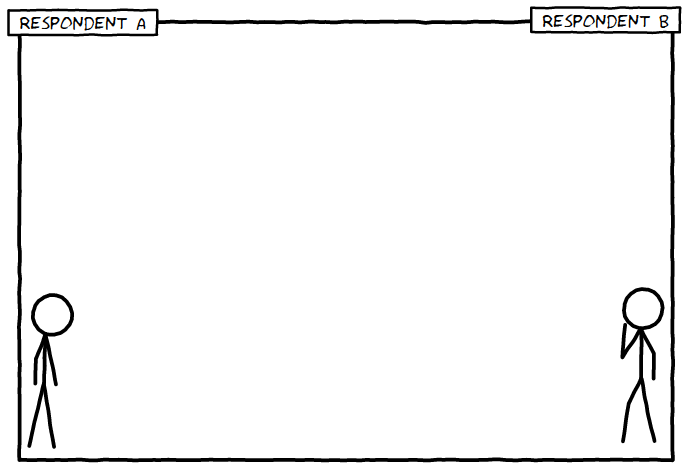
\includegraphics[width=.9\textwidth]{fig/Respondents_empty.png}};
            \node[align=center] at (image.center) {\Large \emph{Measuring Discursive Sophistication}};
        \end{tikzpicture}
    \end{center}
\end{frame}

% INTRODUCTION
% Work on transition for discursive sophistication

\begin{frame}{Discursive Sophistication
	\only<1-3>{-- Components}\only<4-5>{-- Structural Topic Model}\label{overview_stm}\only<6->{-- Components}}
\begin{center}
        \begin{tikzpicture}
            \node<1-4>[anchor=south west,inner sep=0] (image) at (0,0) {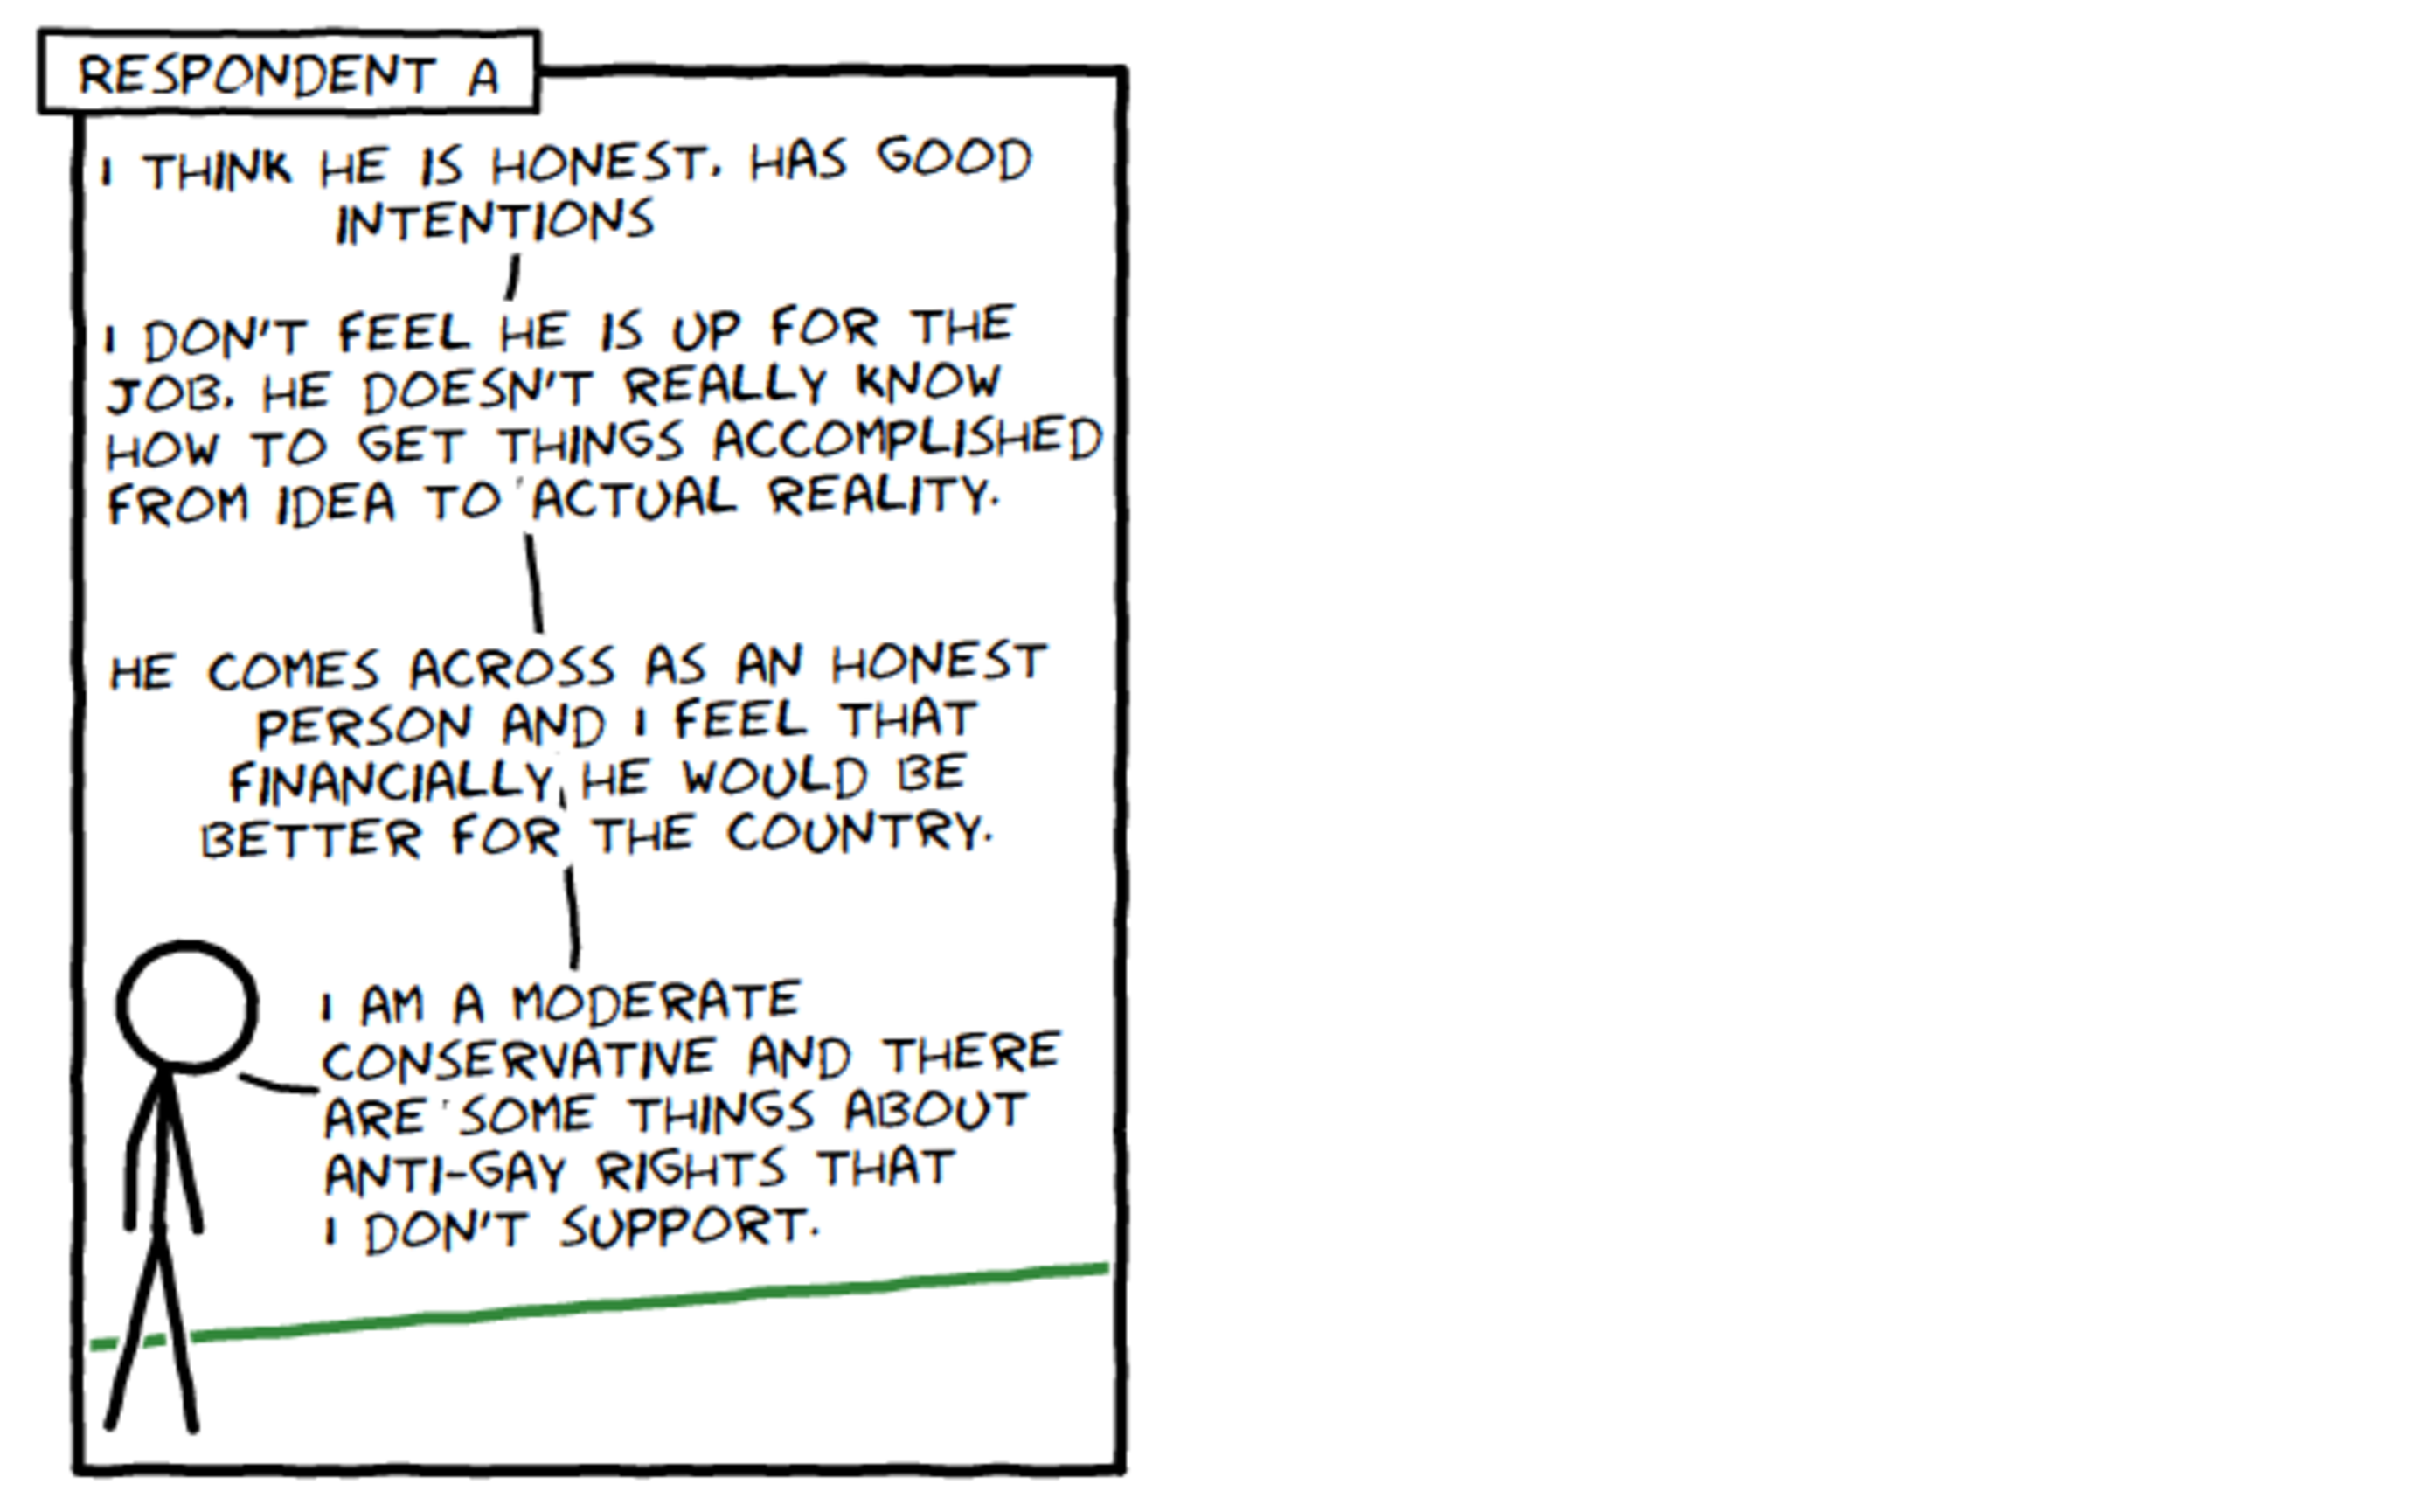
\includegraphics[width=\textwidth]{fig/lda_empty.pdf}};
            \node<2-3>[align=left] (image) at (9,4) {
            	\only<2->{\emph{\faCaretRight} \hyperlink{opinionation}{\emph{Opinionation}}\\
            	Does a respondent discuss all questions?}\\\\
            	\only<3->{\emph{\faCaretRight} \hyperlink{elaboration}{\emph{Considerations}}\\
            	How many topics are mentioned?}\\\\
            	\only<5->{\emph{\faCaretRight} \hyperlink{eloquence}{\emph{Word Choice}}\\
            	Are terms highly descriptive of topics?}
        		};
            \node<4>[align=left] (image) at (9,4) {
            \emph{Processing} open-ended responses:\\
            \emph{\faCaretRight} Automatic spell checking\\
            \emph{\faCaretRight} Lower case\\
            \emph{\faCaretRight} Stopwords, Numbers, Punctuation\\
            \emph{\faCaretRight} Stemming\\
            \emph{\faCaretRight} Infrequent terms\\
            \emph{\faCaretRight} Aggregation \vspace{1em}\\
            \emph{\faArrowRight} \emph{Structural topic model}\\ {\footnotesize\citep{roberts2014structural}}};
            \node<5>[anchor=south west,inner sep=0] (image) at (0,0) {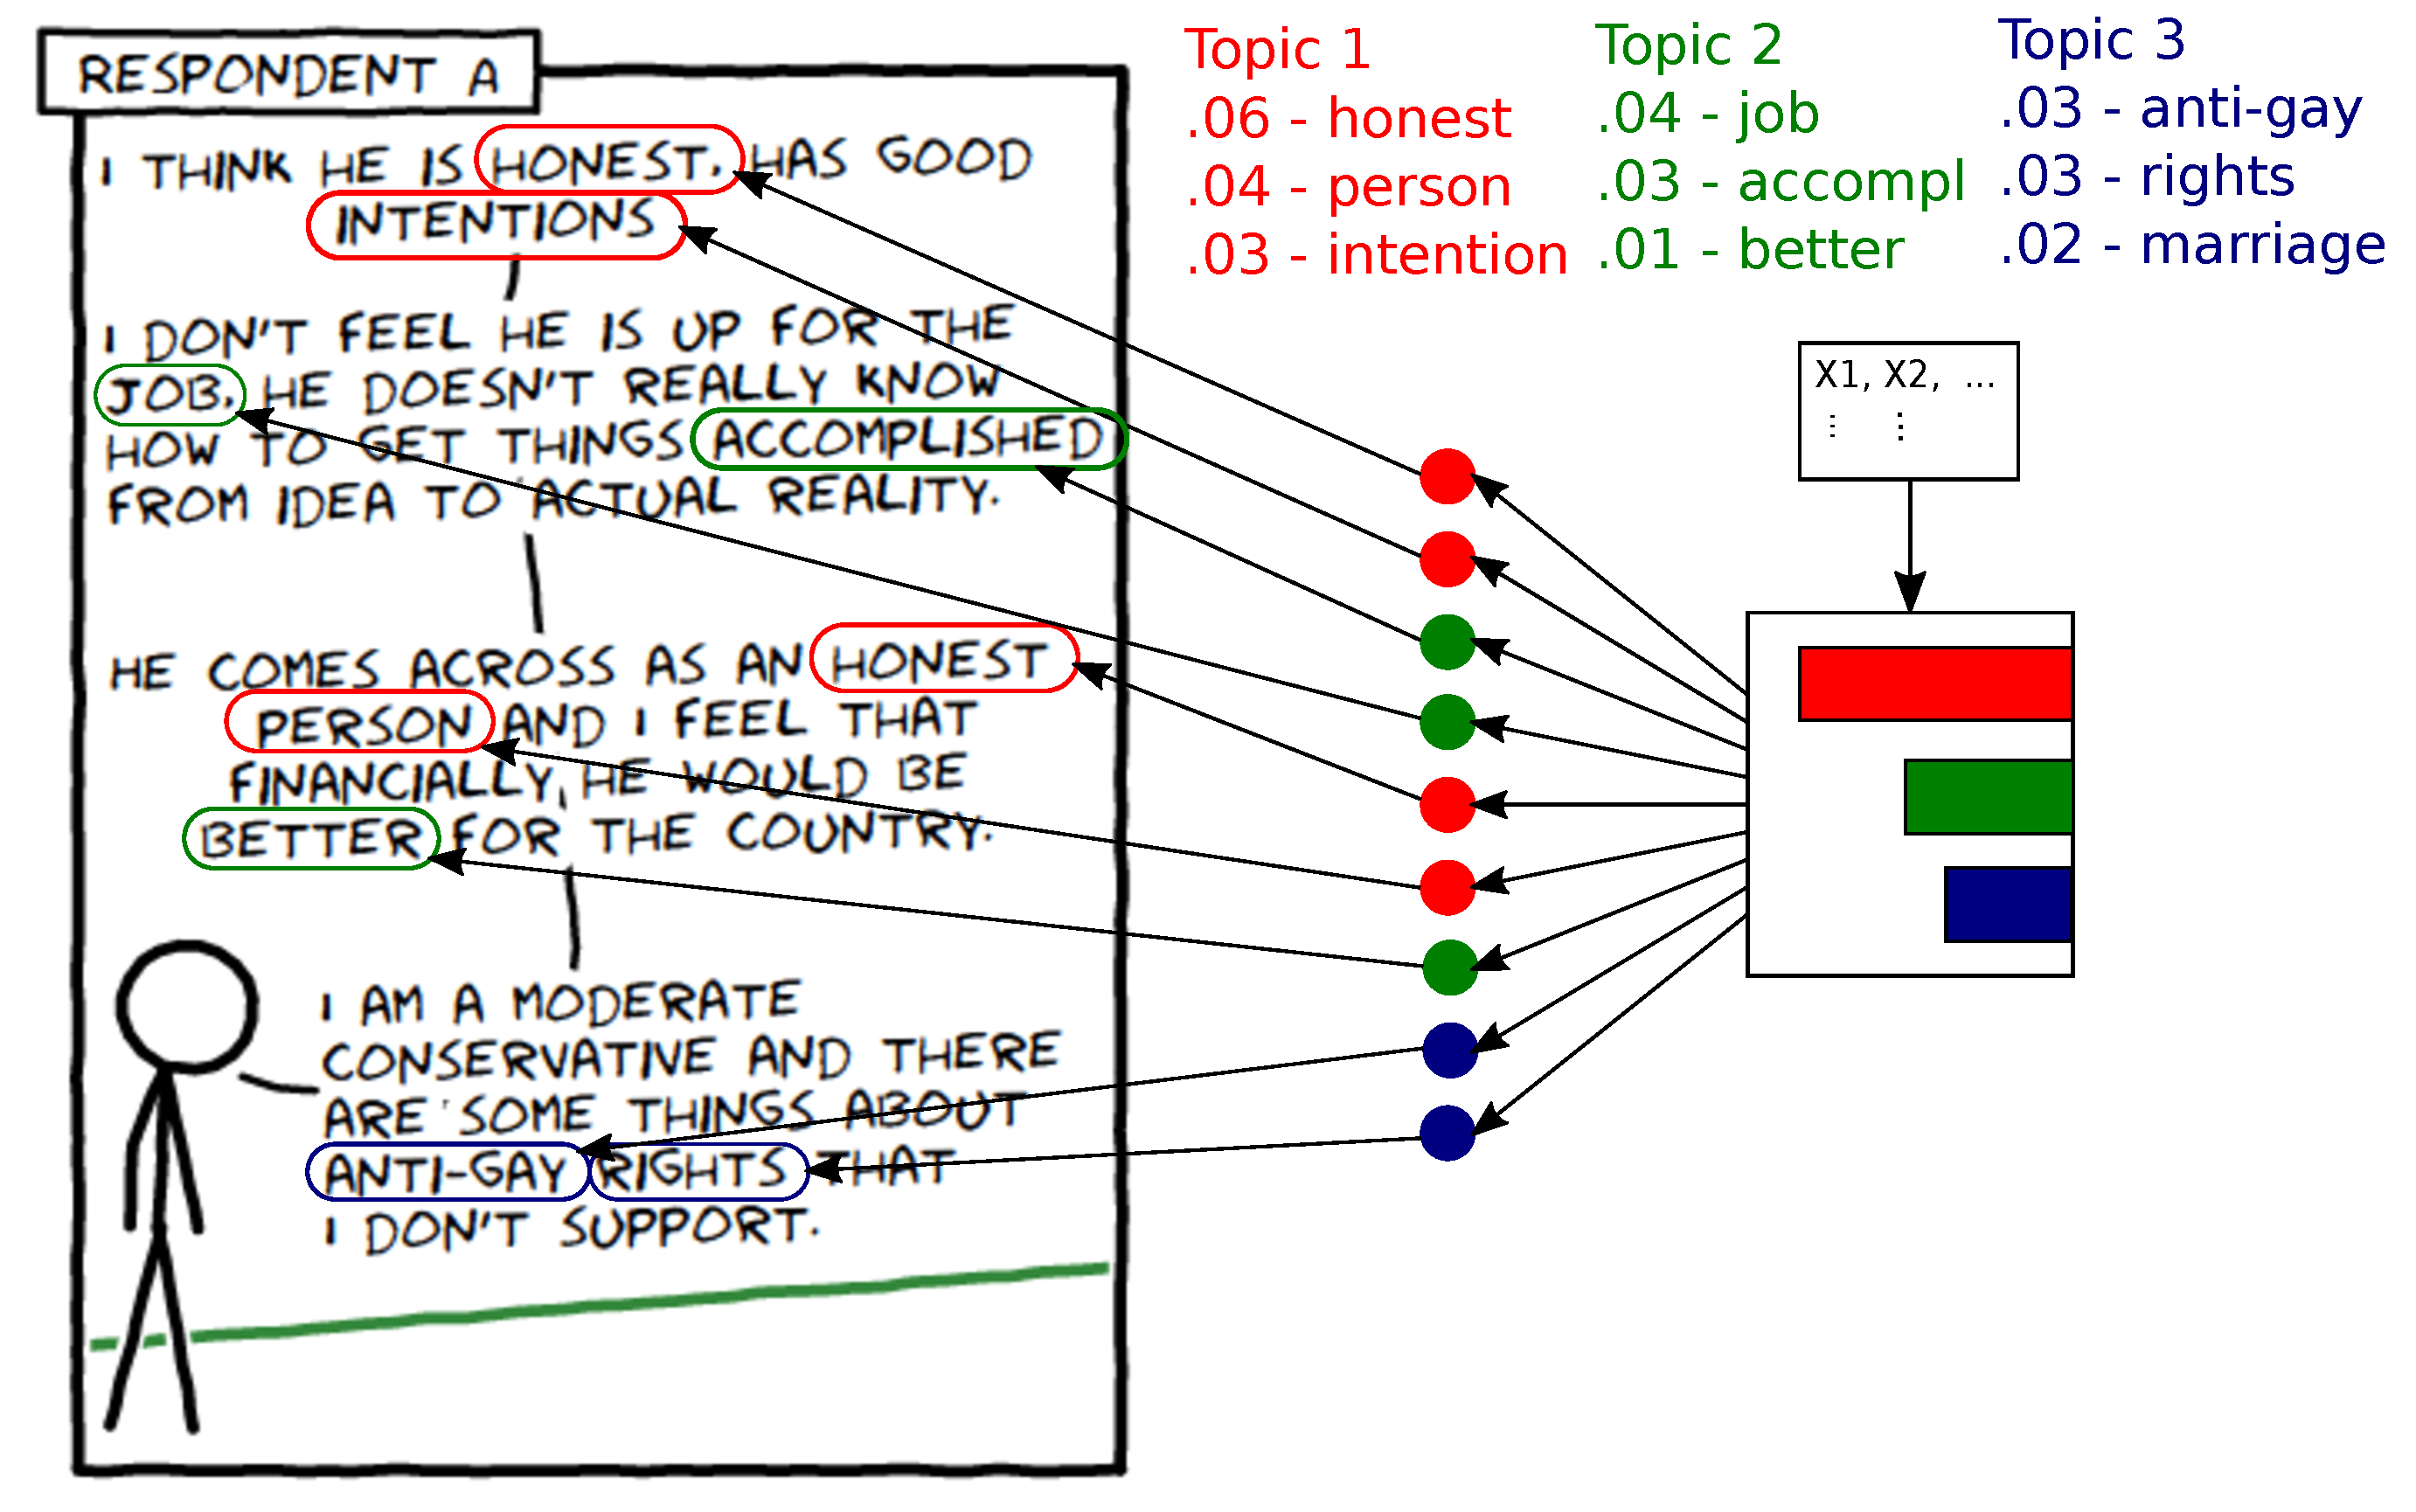
\includegraphics[width=\textwidth]{fig/lda.pdf}};
            \node<6->[anchor=south west,inner sep=0] (image) at (0,0) {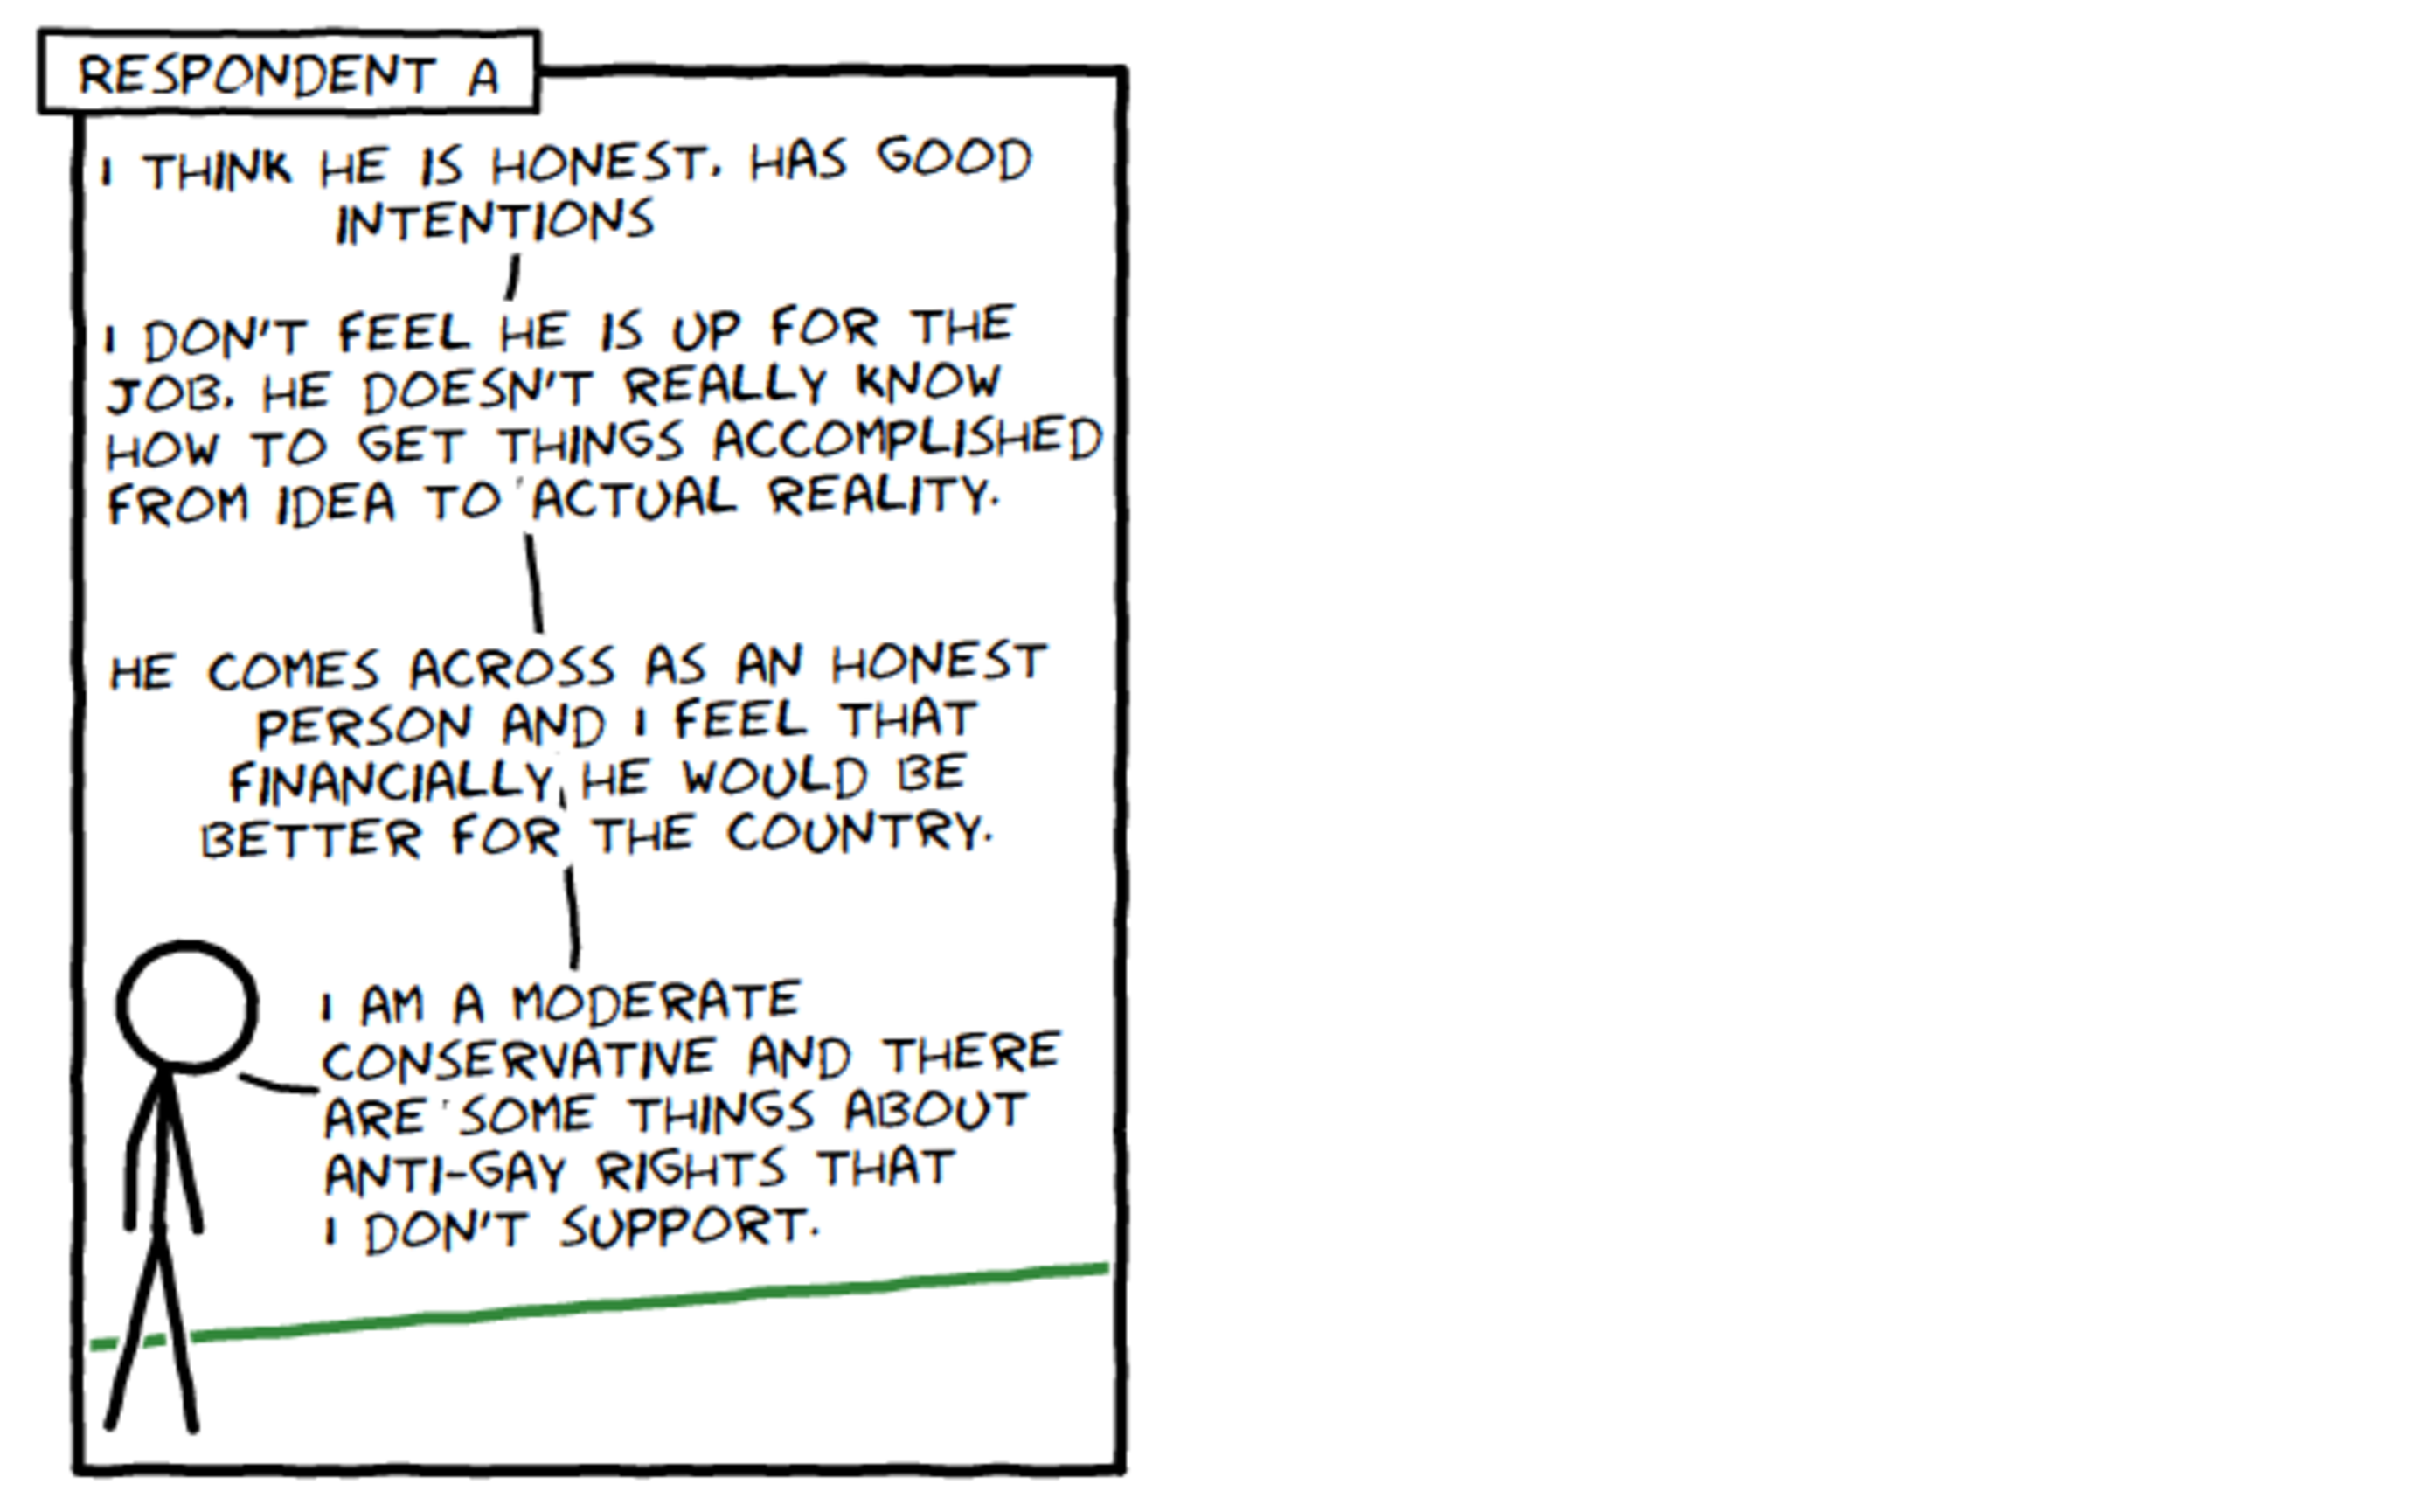
\includegraphics[width=\textwidth]{fig/lda_empty.pdf}};
            \node<6->[align=left] (image) at (9,4) {
            	\only<6->{\emph{\faCaretRight} \hyperlink{opinionation}{\emph{Opinionation}}\\
            		Does a respondent discuss all questions?}\\\\
            	\only<6->{\emph{\faCaretRight} \hyperlink{elaboration}{\emph{Considerations:}}\\
            		How many topics are mentioned?}\\\\
            	\only<6->{\emph{\faCaretRight} \hyperlink{eloquence}{\emph{Word Choice:}}\\
            		Are terms highly descriptive of topics?}
            };
        \end{tikzpicture}
    \end{center}
%\visible<2>{\flushright\small \cite{roberts2014structural}}
%\flushright{\footnotesize\texttt{\textcolor{gray}{\hyperlink{components}{[back]}}}}
\end{frame}

%\begin{frame}{Discursive Sophistication -- Components}\label{components}
%\visible<1->{Extracted \emph{Quantities}:
%\begin{enumerate}
%\item \hyperlink{opinionation}{\emph{Opinionation:}} Does a respondent discuss all questions?
%\item<2-> \hyperlink{elaboration}{\emph{Considerations:}} How many topics are mentioned?
%\item<4-> \hyperlink{eloquence}{\emph{Word Choice:}} Are terms highly descriptive of topics? 
%
%\end{enumerate}}
%
%\only<3>{
%\begin{textblock*}{54mm}(7mm,0.65\textheight)
%\begin{exampleblock}{Few Considerations}
%    {\color{green!50!black}{Represents all people.}}
%    \\{\color{red}{Represent the rich.}}
%    \\{\color{green!50!black}{Represents the working class.}}
%    \\{\color{red}{Represents the wealthy.}}
%\end{exampleblock}
%\end{textblock*}
%\begin{textblock*}{54mm}(67mm,0.65\textheight)
%\begin{exampleblock}{Many Considerations}
%	{\color{green!50!black}{Everything.}}
%	\\{\color{red}{Attitude toward women's rights, view on taxes mainly.}}
%	\\{\color{green!50!black}{Has more people that I trust.}}
%	\\{\color{red}{Too conservative.}}
%\end{exampleblock}
%\end{textblock*}
%} % Answers between 10 and 20 terms, min vs. max elaboration
%
%\only<5>{
%\begin{textblock*}{54mm}(7mm,0.65\textheight)
%\begin{exampleblock}{Low Descriptiveness}
%  enthus\\standoffish\\endless
%\end{exampleblock}
%\end{textblock*}
%\begin{textblock*}{54mm}(67mm,0.65\textheight)
%\begin{exampleblock}{High Descriptiveness}
%  health\\tax\\economi
%\end{exampleblock}
%\end{textblock*}
%} % Individual terms ranked highest and lowest on distinctiveness
%
%\end{frame}
%% add examples for each dimension here


%\subsection{Relationship Between Individual Sophistication Components}
\begin{frame}{\hyperlink{corplot}{Discursive Sophistication -- Components (2012 ANES)}}\label{corplot_components}
\begin{center}
        \begin{tikzpicture}
            \node<1>[anchor=south west,inner sep=0] (image) at (0,0) {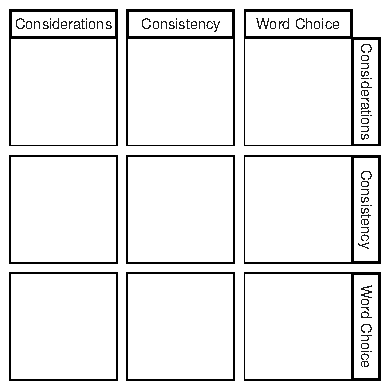
\includegraphics[height=.85\textheight]{../fig/anes2012_corplot_components0.pdf}};
            \node<2->[anchor=south west,inner sep=0] (image) at (0,0) {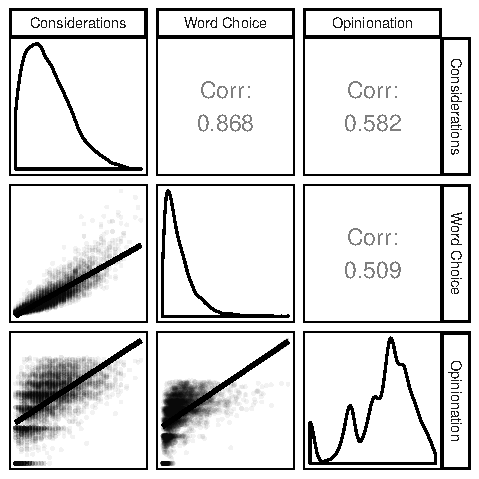
\includegraphics[height=.85\textheight]{../fig/anes2012_corplot_components.pdf}};
            \node<3>[align=center,draw opacity=0,fill opacity=0.8,text opacity=1, white, fill=beamer@sbred] at (image.center) {Discursive Sophistication\\=\\ $\tfrac{1}{3}$(Opinionation + Considerations + Word Choice)};
        \end{tikzpicture}
    \end{center}
%\visible<2>{\flushright\small \cite{roberts2014structural}}
%\flushright{\footnotesize\texttt{\textcolor{gray}{\hyperlink{components}{[back]}}}}
\end{frame}




\section{Validation: Discursive Sophistication and Political Competence}
\subsection{Validation using 2012 ANES}
% Here, we will look at political sophistication and competence

\begin{frame}\centering\vfill
    \begin{center}
        \begin{tikzpicture}
            \node[anchor=south west,inner sep=0] (image) at (0,0) {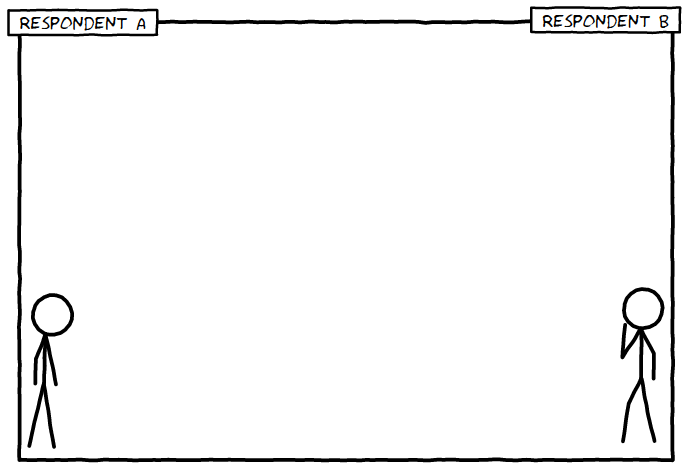
\includegraphics[width=\textwidth]{fig/Respondents_empty.png}};
            \node<2->[anchor=south west,inner sep=0] (vote) at (1.5,5) {
\includegraphics[width=.4\textwidth]{fig/Voting.jpg}};
            \node<3->[anchor=south west,inner sep=0] (protest) at (4.6,1.5) {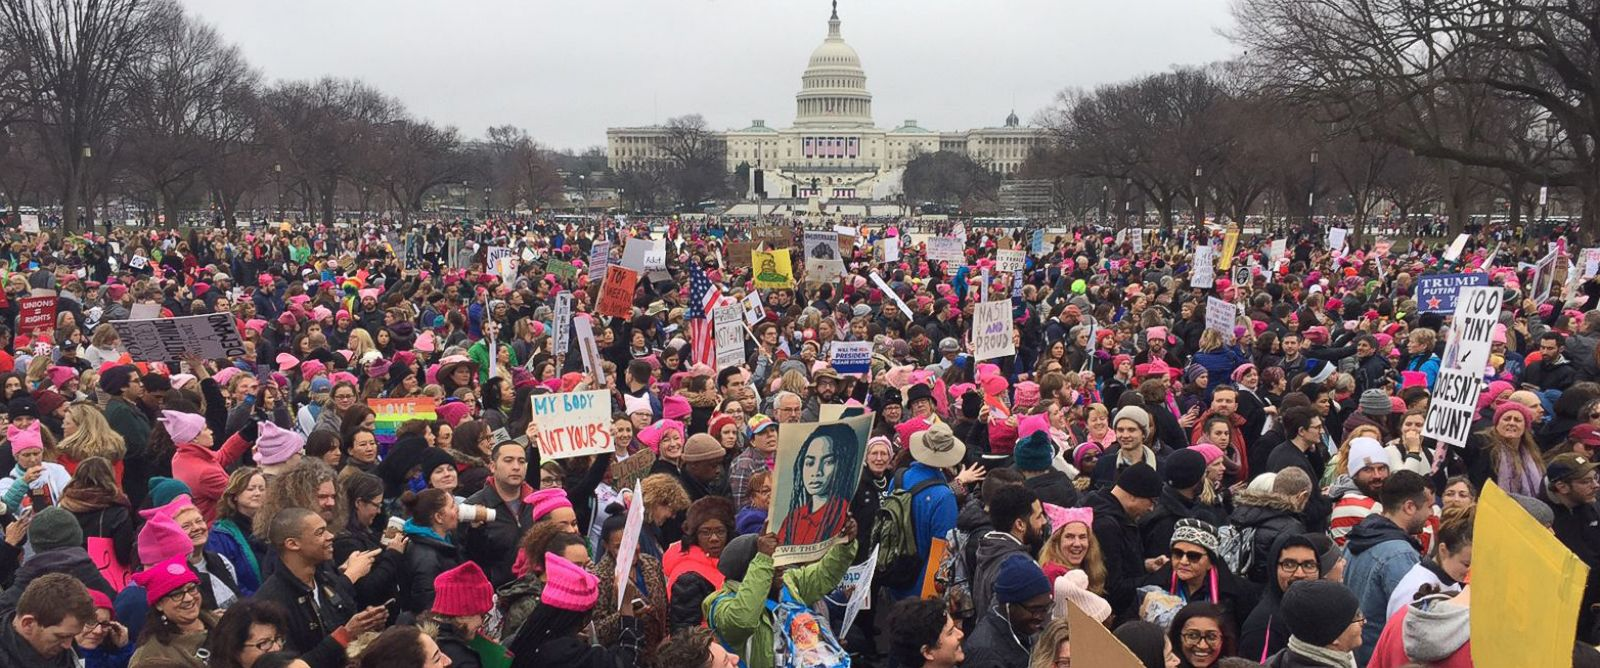
\includegraphics[width=.5\textwidth]{fig/GTY-womens-march.jpg}};
            \node<4->[anchor=south west,inner sep=0] (thinking) at (1.5,1.5) {
\includegraphics[width=.25\textwidth]{fig/gear-head-blue.png}};
            \node<5->[anchor=south west,inner sep=0] (influence) at (6.5,4.5) {
\includegraphics[width=.3\textwidth]{fig/Influence.png}};
            \node<6->[align=center,draw opacity=0,fill opacity=0.8,text opacity=1, white, fill=beamer@sbred] at (image.center) {\large Validation\\\Large 2012 American National Election Study\\\vspace{1em}\\N = 5914 (2054 f2f + 3860 online)};
        \end{tikzpicture}
    \end{center}
\end{frame}
%\item Non-response: 417, Spanish: 228

\begin{frame}{\hyperlink{engagement_joint}{Engagement and Participation}}\label{engagement}
  \begin{figure}
  \only<1>{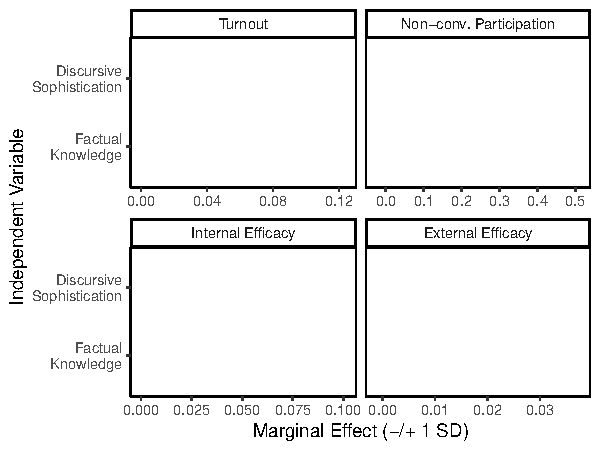
\includegraphics{../fig/knoweff_pres0.pdf}}
  \only<2>{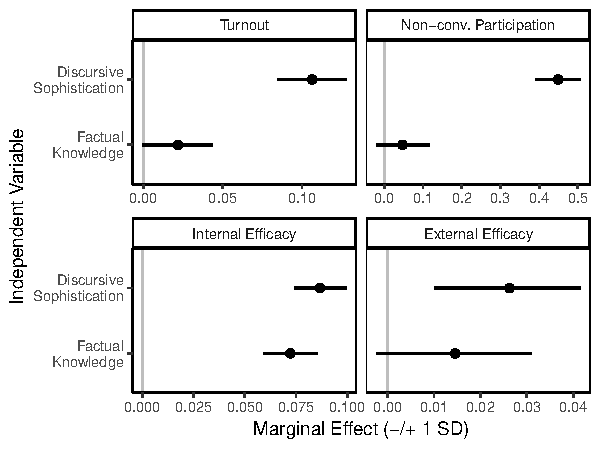
\includegraphics{../fig/knoweff_pres1.pdf}}
  \end{figure}
\end{frame}
% DISCUSS:
% Discursive sophistication is associated with:
% - \hyperlink{hetreg}{more precise candidate and party \emph{placements} on multiple \emph{policy} issues.
% -\hyperlink{prepost}{higher likelihood that citizens \emph{voted} according to their \emph{initial intention} at the time of the \emph{pre-election} interview.







\section{Application: Assessing the Gender Gap}
\subsection{Previous Research on Gender Differences in Knowledge}
% Now I want to show you why this matters
% This application challenges a common finding in political science and public opinion research, namely that women know significantly less about politics than men. Some studies attribute this difference to a relative lack in resources like education, or a more general disdain for politics among women. However, others argued that the gender gap might be an artifact due to differential propensities to guess or the fact that knowledge questions do not address gender relevant knowledge. I examine the gender gap by proposing a new measure of political sophistication that focuses on how individuals describe their political attitudes and beliefs in their own words.
% Example for gender gap: Verba, Burns, Schlozman (1997), Mondak


\begin{frame}\centering\vfill
    \begin{center}
        \begin{tikzpicture}
            \node[anchor=south west,inner sep=0] (image) at (0,0) {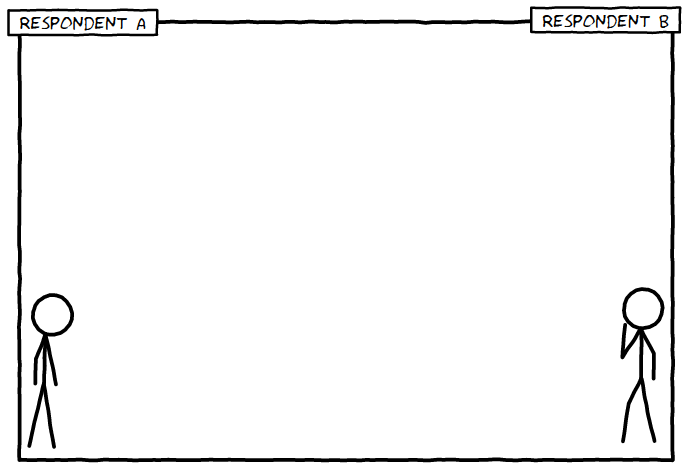
\includegraphics[width=\textwidth]{fig/Respondents_empty.png}};
            \node<2->[anchor=south west,inner sep=0] (vote) at (3.6,1.5) {
\includegraphics[width=.4\textwidth]{fig/Mind_the_gap1.jpg}};
            \node<3->[align=center,draw opacity=0,fill opacity=0.8,text opacity=1, white, fill=beamer@sbred] at (image.center) {\large Application
            \\\Large Assessing the Gender Gap
            \\\Large in Political Sophistication
            \\\vspace{1em}\\ (2012 \& 2016 ANES + 2015 YouGov)};
        \end{tikzpicture}
    \end{center}
\end{frame}
% Mention that results replicate in the remaining datasets


\begin{frame}{Previous Research on Gender Differences in Knowledge}
\visible<1->{\emph{General finding}: Women score \emph{lower} than men on \emph{conventional} measures of\\ \emph{political knowledge}
%\begin{itemize}\footnotesize
%\item \cite{converse1964nature}, \cite{verba1997knowing}
%% Converse: found gap, Verba: cannot be reduced, general distaste, Dow: women benefit differently from factors that increase knowledge
%\end{itemize}
}
\vspace{1em}
\visible<2->{\begin{center}
\emph{\faArrowRight}\hspace{1em} ``One of the \emph{most robust} findings in the study of political behavior.'' {\footnotesize\cite{dow2009gender}}
\end{center}}
\vspace{2em}
\visible<3->{\emph{Explanation 1:} Personality characteristics
%\begin{itemize}\footnotesize
%\item \cite{mondak2004knowledge}, \cite{mcglone2006stereotype}
%%Mondak: propensity to guess; McGlone: stereotype threat; Lizotte: propensity to guess due to risk aversion
%\end{itemize}
}\\\vspace{1em}
\visible<4->{\emph{Explanation 2:} Question content / gender-relevant knowledge
%\begin{itemize}\footnotesize
%\item \cite{stolle2010women}, \cite{dolan2011women}, \cite{jerit2017revisiting}
%% Stolle: practical issues (benefits/services); Dolan: women's representation; Jerit: Closing gap through learning)
%\end{itemize}
}
\end{frame}


\subsection{Gender Differences in Sophistication}

\begin{frame} %[allowframebreaks]
\frametitle{Gender Differences in Sophistication}
  \begin{figure}
  \only<1>{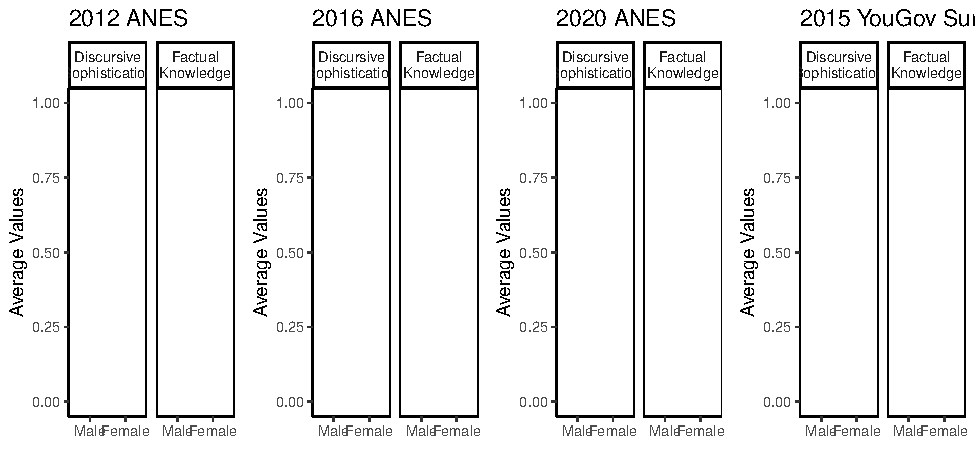
\includegraphics[width=1\textwidth]{../fig/meandiff_pres_empty.pdf}}
  \only<2>{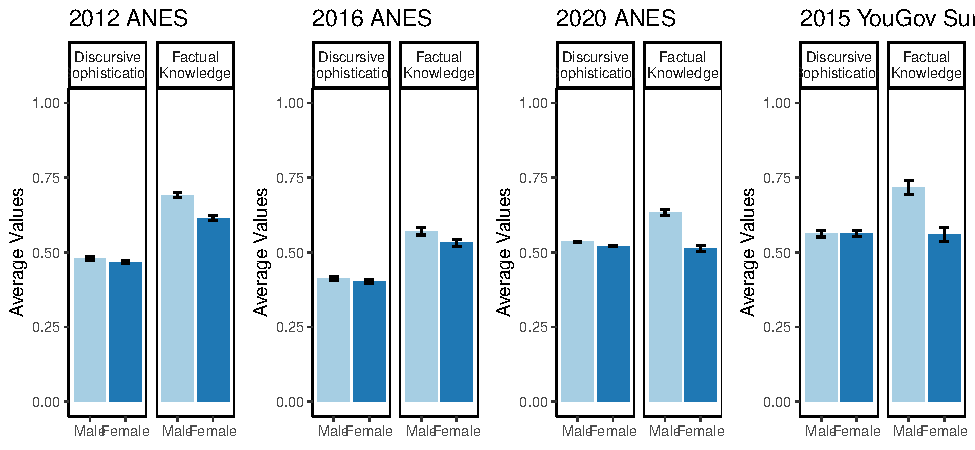
\includegraphics[width=1\textwidth]{../fig/meandiff_pres.pdf}}
  \end{figure}
\end{frame}

\begin{frame} %[allowframebreaks]
\frametitle{Explaining the Gender Gap in Political Knowledge}
\begin{figure}
	\only<1>{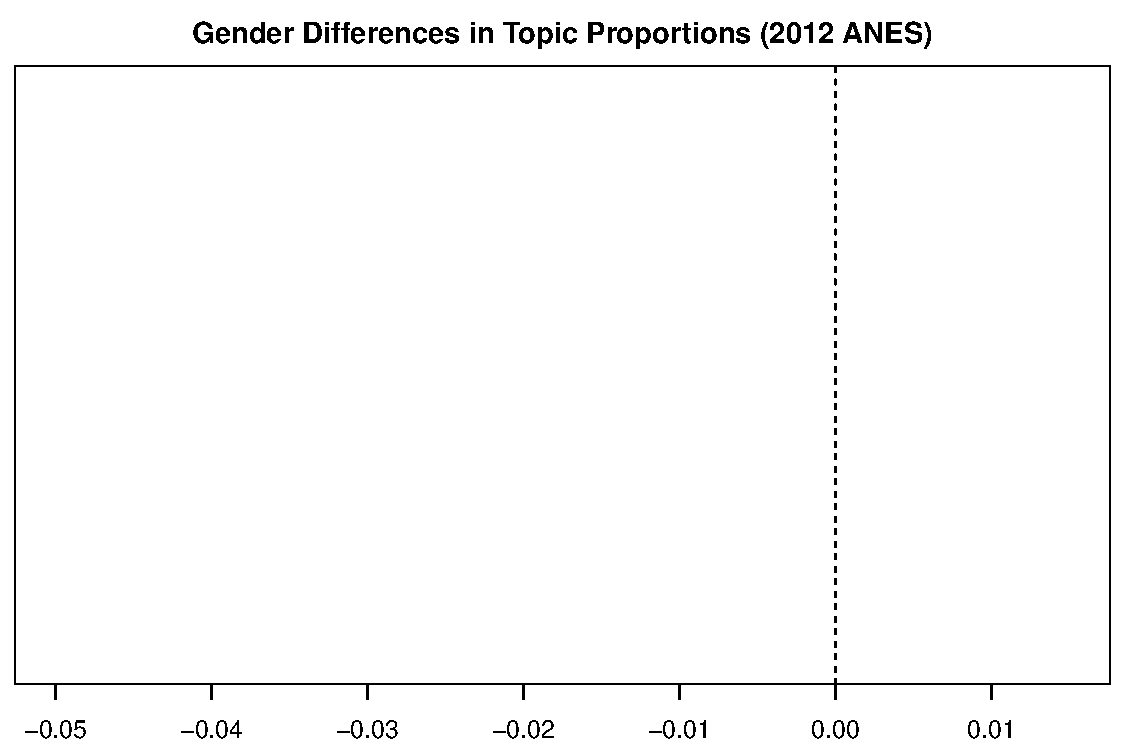
\includegraphics[width=1\textwidth]{../fig/stm_gender_pres0.pdf}}
	\only<2>{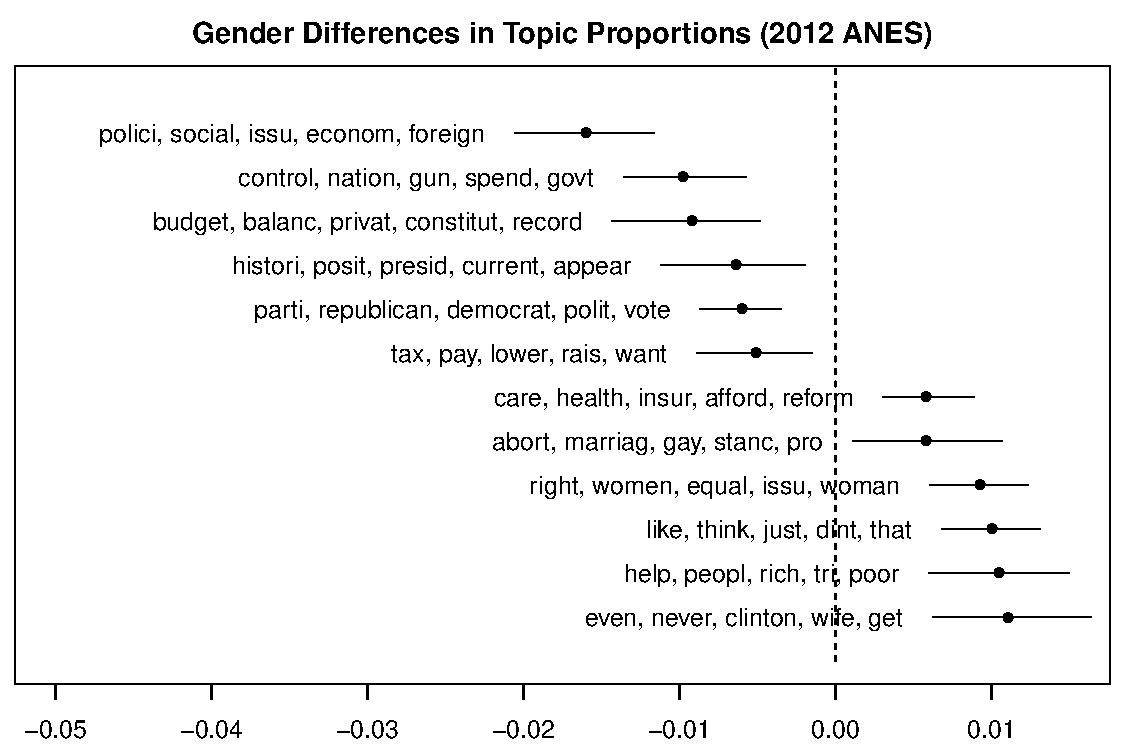
\includegraphics[width=1\textwidth]{../fig/stm_gender_pres1.pdf}}
\end{figure}
\end{frame}

% TODO: add the yougov study as a replication



\section{Conclusion}
\begin{frame}
    \begin{center}
        \begin{tikzpicture}
            \node[anchor=south west,inner sep=0] (image) at (0,0) {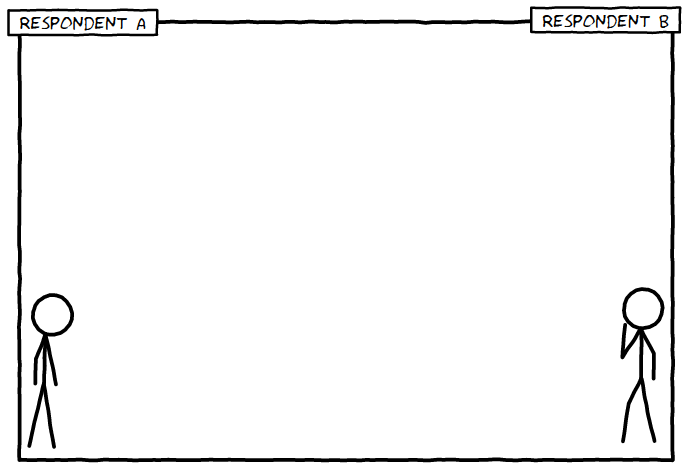
\includegraphics[width=.9\textwidth]{fig/Respondents_empty.png}};
            \node[align=center] at (image.center) {\Large \emph{Conclusion}};
        \end{tikzpicture}
    \end{center}
\end{frame}


\subsection{General Discussion}

\begin{frame}%[allowframebreaks]
  \frametitle{General Discussion}
  \begin{itemize}
\item We observe \emph{theoretically meaningful} variation in the \emph{complexity} of verbatim open-ended responses.
%\item Discursive sophistication and conventional knowledge measures \emph{share a substantial amount of variance}, but they are far from identical.
\item<2->  By directly examining how individuals \emph{justify their attitudes}, we can measure sophistication related to \emph{specific political tasks}.
\item<3-> Discursive sophistication is conceptually closer to the \emph{structure of belief systems} than conventional measures.

\vspace{1em}
\item<4-> Women might score lower than men on \emph{factual knowledge} about political institutions, but there are no differences in the \emph{sophistication} of expressed political attitudes.
%\begin{center}\emph{\texttt{\#WomenAlsoKnowStuff}}\end{center}
\end{itemize}
\end{frame}
%Information vs. competence argument by Lupia!!


\begin{frame}{Illustration -- Who scores higher on political knowledge?}
    \begin{center}
        \begin{tikzpicture}
            \node[anchor=south west,inner sep=0] (image) at (0,0) {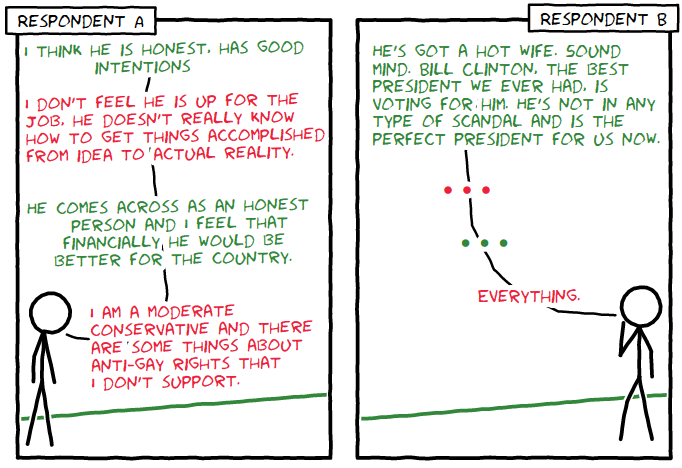
\includegraphics[width=.9\textwidth]{fig/Respondents8.png}};
            \node<2->[anchor=south west,inner sep=0] (image) at (1.4,2) {
\includegraphics[width=.3\textwidth]{fig/We_Can_Do_It!.jpg}};
            \node<3->[anchor=south west,inner sep=0] (image) at (5.8,3.5) {
\includegraphics[width=.3\textwidth]{fig/skinny-man.jpg}};
        \end{tikzpicture}
    \end{center}
\end{frame}


\begin{frame}%[allowframebreaks]
  \begin{center}
  \large{Thank you very much for your attention!}\\ \vspace{2em}
  Manuscript and code available at:\\
  %\emph{\texttt{https://github.com/pwkraft/mft}}\\
  \emph{\texttt{https://github.com/pwkraft/knowledge}}\\ \vspace{2em}
  Comments, questions?\\
  \emph{\faEnvelopeO\hspace{.5em}\texttt{kraftp@uwm.edu}}\\\vspace{2em}
  \emph{\faGlobe\hspace{.5em}\texttt{pwkraft.github.io}}\\
  \emph{\faTwitter\hspace{.5em}\texttt{@patrickwkraft}}\\
  \end{center}
\end{frame}

% RESPONSE to question about rationalization:
% I think that is a fair point and that is something that we definitely have to take into account when interpreting these results. But I would think of it as not being a bug but rather a feature of the approach. In Druckman's 2014 article on the "Pathologies of Studying Public Opinion", he makes the argument that it is unclear whether factual information is necessary for people to have quality opinions. Instead, he argues that we should look at the process by which people come to their opinions, and what he means is whether people are motivated to come to an accurate opinion. In psychology, accuracy motivation is often induced by asking people to justify their opinions. So I think it makes sense to examine how well they are sophisticated in providing these justifications in order to assess whether their opinions are indeed well-grounded and based on careful consideration.

\section*{Content}
\label{sec:main-content}
\begin{frame}%[allowframebreaks]
\frametitle{Content}
\tableofcontents%[hideallsubsections]
\end{frame}

\appendix
\section*{Appendix Content}
\label{sec:appendix-content}
\begin{frame}%[allowframebreaks]
\frametitle{Appendix Content}
\small\tableofcontents %[hideallsubsections]
\end{frame}
\section{Measuring Discursive Sophistication}

\subsection{Item Wording}
\begin{frame}{Factual Knowledge Questions}
\begin{itemize}
\item \emph{\cite{carpini1993measuring}}: House majority, veto override percent, party ideological location, judicial review, identifying the vice president
\item \emph{2012 ANES}: Number of times president can be elected, size of federal deficit, full term of senator, meaning of medicare, federal government spending
\item \emph{2015 YouGov}: Speaker of the House, TTIP, Chair of Federal Reserve Board, unemployment rate, veto override percent, common core, largest electricity source, Senate majority
\end{itemize}
\end{frame}
% Carpini: 780 citations

\begin{frame}{Open-Ended Items: 2012 ANES}
\begin{itemize}
\item Is there anything in particular about [CANDIDATE] that might make you want to vote for him? [...] What is that?
\item Is there anything in particular about [CANDIDATE] that might make you want to vote against him? [...] What is that?
\item Is there anything in particular that you like about [PARTY]? [...] What is that?
\item Is there anything in particular that you don't like about [PARTY]? [...] What is that?
\end{itemize}
\end{frame}

\begin{frame}{Open-Ended Items: 2015 YouGov}
\begin{itemize}
\item Do you favor or oppose stricter gun control laws? [...] Still thinking about the question you just answered, what thoughts came to mind while you were answering that question? Please try to list everything that came to mind.
\item Thinking about the mass shootings that have occurred in the U.S. in the last few years, what factors do you think are responsible for the shootings?
\item Do you support or oppose the health care law passed by the President and Congress in 2010?
[...] Still thinking about the question you just answered, what thoughts came to mind while you were answering that question? Please try to list everything that came to mind.
\item For decades, experts have observed that the United States spends far more per person on health care than any other country. However, the U.S. falls behind on most measures of health care outcomes, such as life expectancy. What factors do you think are responsible for the state of our health care system?
\end{itemize}
\end{frame}

\begin{frame}{Open-Ended Items: 2008--2012 Swiss Referenda}
\begin{itemize}
\item Which are your main reasons for accepting/rejecting the proposal [X]?
\item What are additional reasons for accepting/rejecting the proposal [X]?
\end{itemize}
\end{frame}

\subsection{Opinionation}
\begin{frame}{\hyperlink{components}{Opinionation}}\label{opinionation}\centering
\emph{Opinionation$_i$} = $\dfrac{-\sum_{j=1}^J p_{ij} \ln p_{ij}}{\ln J}$
\vspace{1em}\\
\begin{tabular}{lp{9cm}}
	\toprule
	$i$ & Respondent \\
	$j \in \{1,...,J\}$ & Open-ended items \\
	$p_{ij}$ & Proportion of words in the response of individual $i$ to question $j$ relative to the overall size of the individual's response\\
\end{tabular}
\end{frame}

\subsection{Considerations}
\begin{frame}{\hyperlink{components}{Considerations}}\label{elaboration}\centering
\emph{Considerations}$_i$ = $\dfrac{|\mathcal{T}^*_i|}{\max|\mathcal{T}^*_i|}$
\vspace{1em}\\
\begin{tabular}{lp{8.5cm}}
\toprule
$i$ & Respondent \\
$\mathcal{T}^*_i $ & Topic representation of response set $\mathcal{W}_i$, such that $w\rightarrow t^*\forall w \in \mathcal{W}_i$ \\
$w \in \mathcal{W}_i$ & Individual word $w$ in response set $\mathcal{W}_i$\\

$t^* \in \{1,...,T\} $ & Topic $t^*$ out of total number of topics $T$ assigned to $w$ such that $P(t^*|w,X_i) > P(t|w,X_i) \forall t\neq t^*$\\
& $P(t|w,X_i)=\dfrac{P(w|t)P(t|X_i)}{P(w|X_i)}$ \\
$X_i$ & Covariates used in structural topic model
\end{tabular}
\end{frame}

\subsection{Word Choice}
\begin{frame}{\hyperlink{components}{Word Choice}}\label{eloquence}\centering
\emph{Word Choice$_i$} = $\dfrac{\log\sum_{\mathcal{W}_i} P(w|t^*)}{\max\left[\log\sum_{\mathcal{W}_i} P(w|t^*)\right]}$
% estimated max topic probabilities of terms
\vspace{1em}\\
\begin{tabular}{lp{8.5cm}}
\toprule
$i$ & Respondent \\
$w \in \mathcal{W}_i$ & Individual word $w$ in response set $\mathcal{W}_i$\\
%$P(w|t^*)$ & Probability of word $w$ for assigned topic $t^*$ \\
$t^* \in \{1,...,T\} $ & Topic $t^*$ out of total number of topics $T$ assigned to $w$ such that $P(t^*|w,X_i) > P(t|w,X_i) \forall t\neq t^*$\\
& $P(t|w,X_i)=\dfrac{P(w|t)P(t|X_i)}{P(w|X_i)}$ \\
%&$P(t|w,X_i)=\dfrac{P(w|t)P(t|X_i)}{\sum_{j=1}^{T}P(w|t_j,X_i)P(t_j|X_i)}$ \\
$X_i$ & Covariates used in structural topic model
\end{tabular}
\end{frame}
% Is a respondent using high probability terms for each topic?



\subsection{}
\begin{frame} %[allowframebreaks]
\frametitle{\hyperlink{corplot_components}{Comparison with Conventional Measures -- 2012 ANES}}\label{corplot}
  \begin{figure}
  %\only<1>{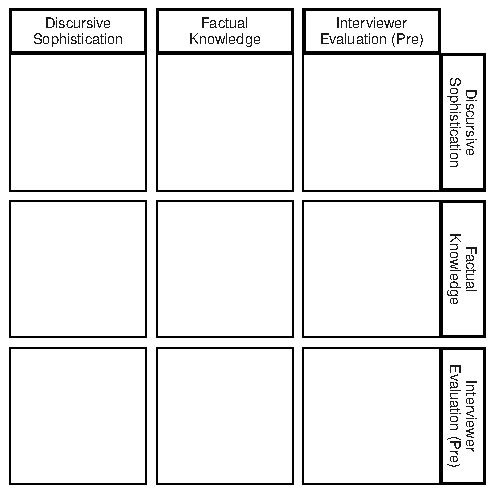
\includegraphics[height=.85\textheight]{fig/corplot_empty.pdf}}
  \only<1>{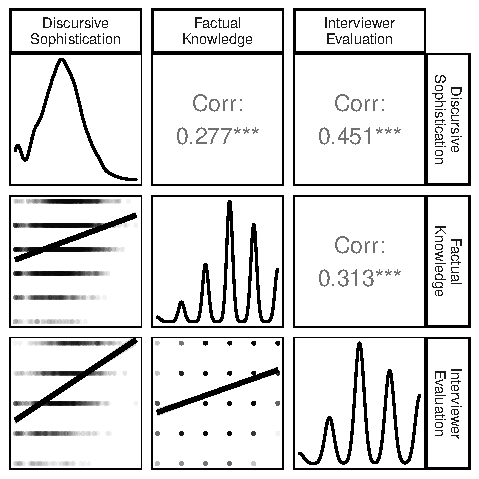
\includegraphics[height=.85\textheight]{../fig/anes2012_corplot.pdf}}
  \end{figure}
\end{frame}
% Now we want to look at desireable characteristics that should be associated with political sophistication -> political engagement as one standard validation check

\section{Additional Results}

\subsection{Topic Proportions -- 2012 \& 2016 ANES}
\begin{frame}{Topic Proportions -- 2012 \& 2016 ANES}\label{stm}
\begin{figure}
	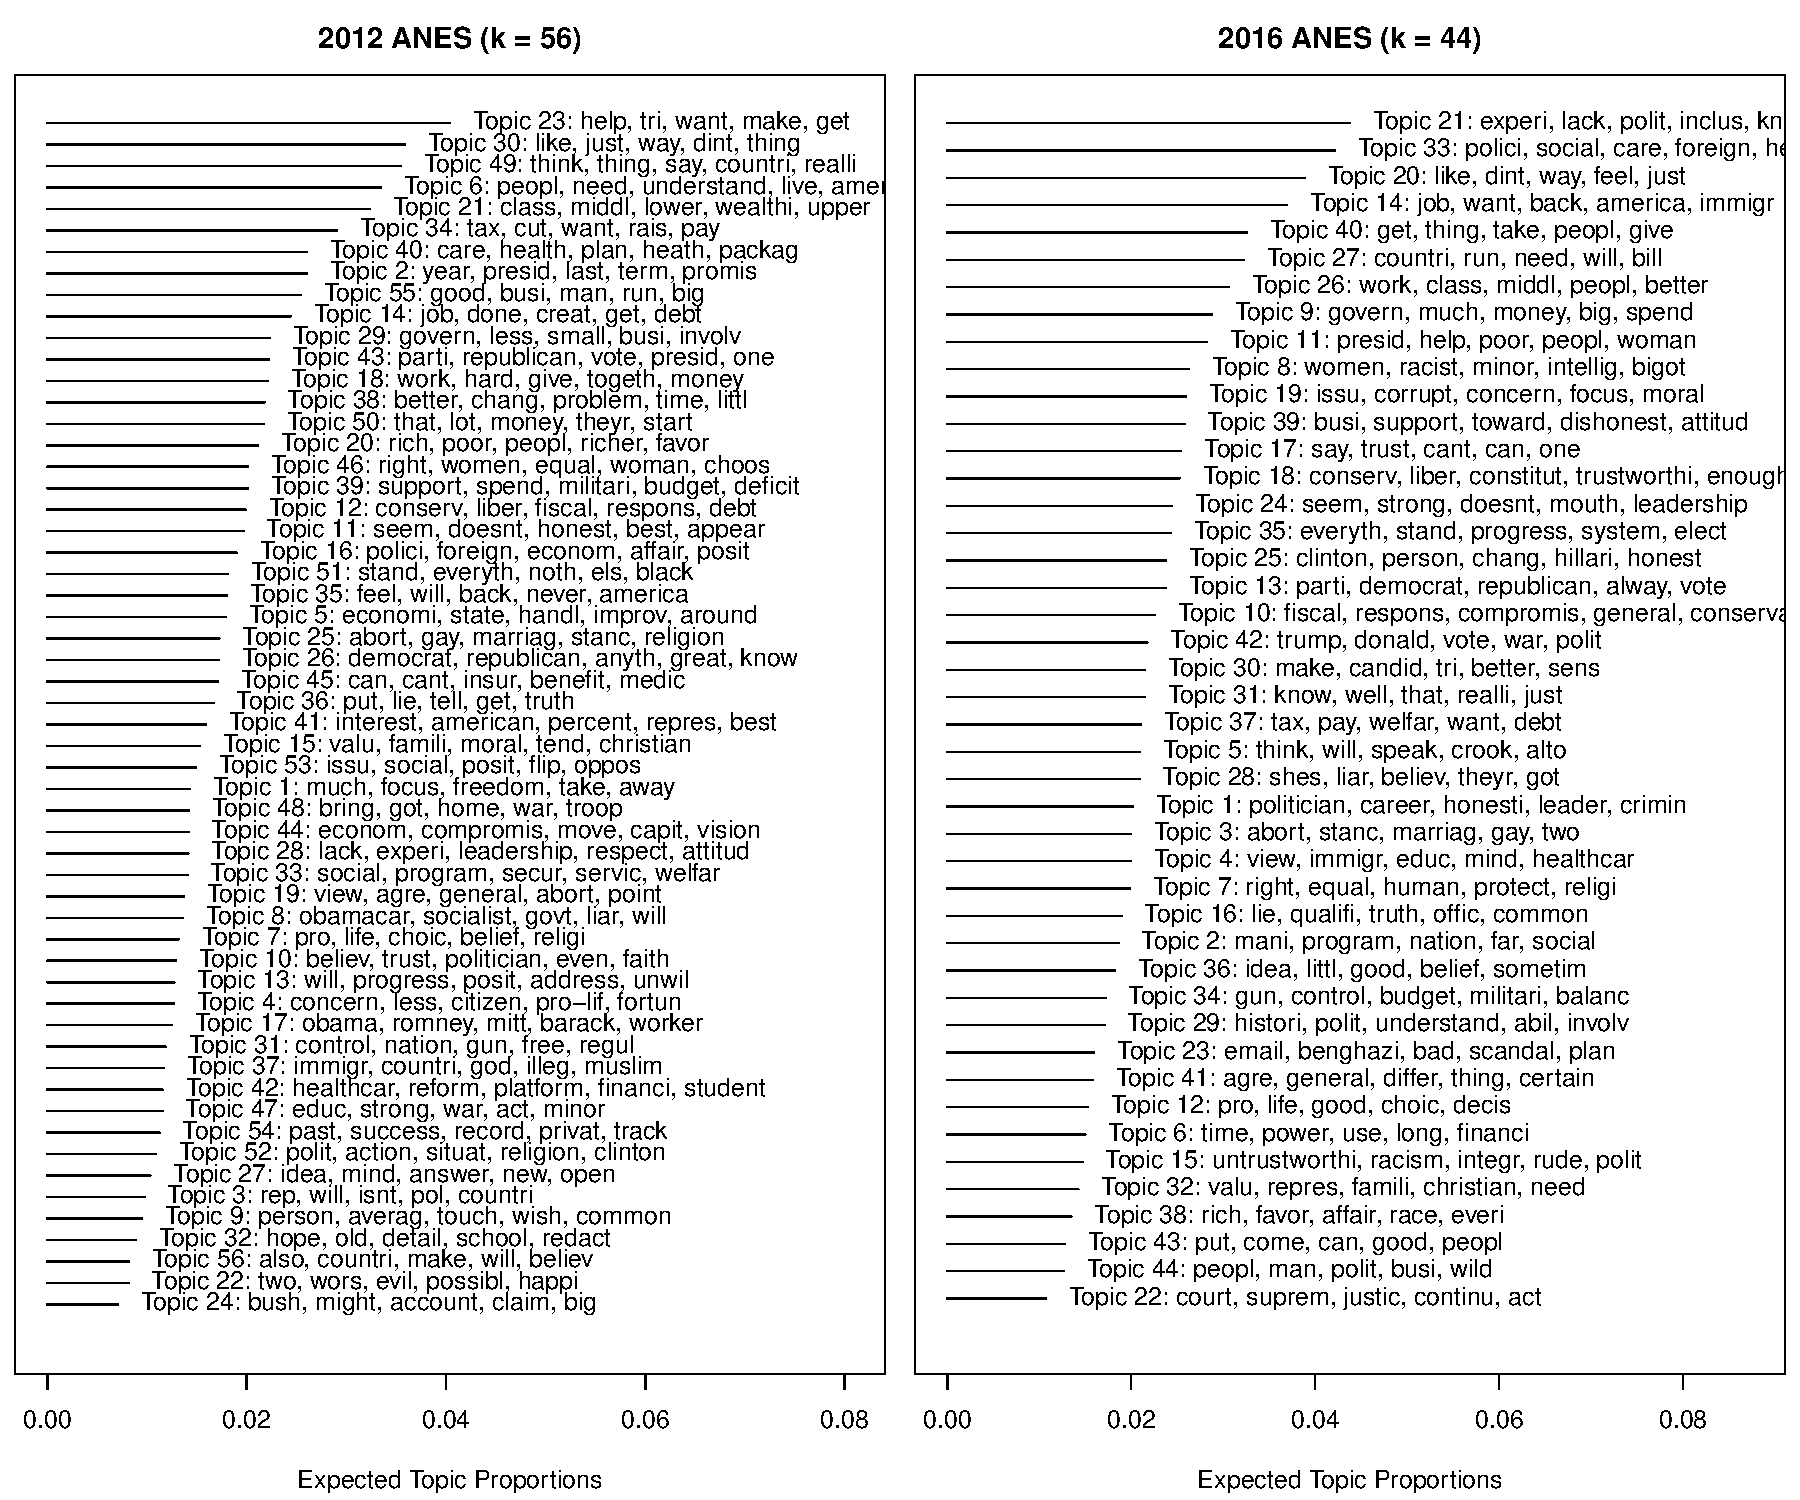
\includegraphics[height=.9\textheight]{../fig/anes_stm_prop.pdf}
\end{figure}
\end{frame}

\subsection{2008--2012 Swiss Referendum Survey}
% Here, we will look at political sophistication and competence
% Manual coding would be the ideal, Colombo as the gold standard

\begin{frame} %[allowframebreaks]
\frametitle{Comparison with Manually Coded Levels of Justification}
\emph{Data source}: 2008--2012 Swiss Referendum Survey, N = 26,621 (phone)
\begin{figure}
	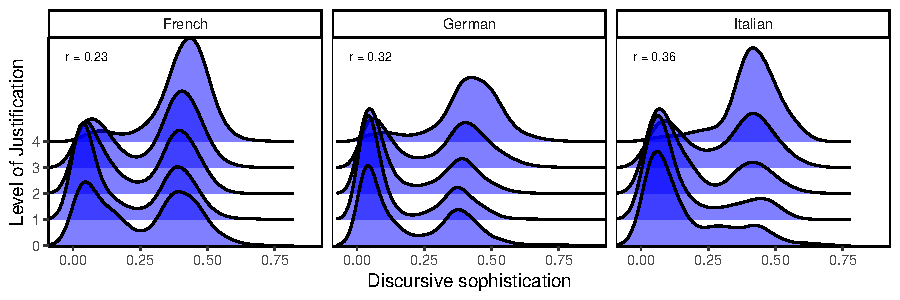
\includegraphics[width=\textwidth]{../fig/swiss_ggridges.pdf}
\end{figure}
\end{frame}
%Non-response: 4,917
% Manually coding would be the gold standard... How would it compare across 3 different languages -> very hard test!!!

\subsection{2015 YouGov Study}
% Here, we will look at political sophistication and competence
% Introduce the main point here!!

\begin{frame} %[allowframebreaks]
\frametitle{\hyperlink{retrieval_joint}{Accurate Information Retrieval}}\label{retrieval}
\emph{Data source}: 2015 YouGov Study, N = 1000 (online)
\begin{figure}
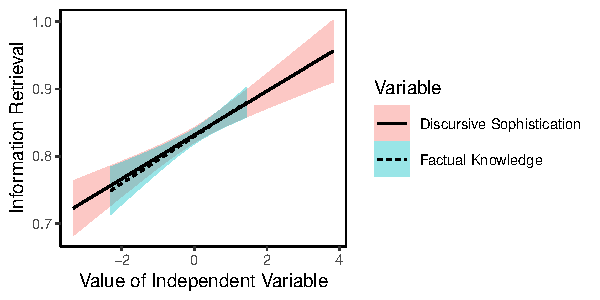
\includegraphics{../fig/yg_disease.pdf}
\end{figure}
\end{frame}
%Non-response: 48


\section{Robustness Checks}

%\subsection{Choosing the Number of Topics}
%\begin{frame}{Choosing the Number of Topics (2012 ANES)}\label{ktopics}
%  \begin{figure}
%  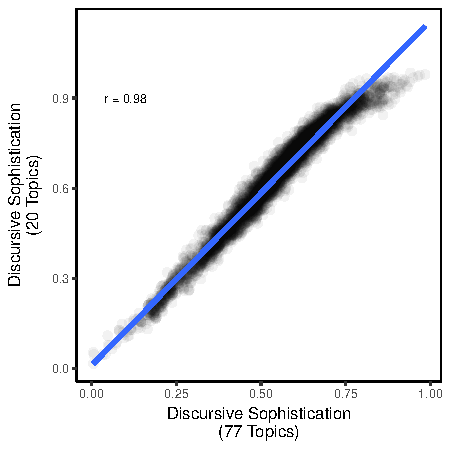
\includegraphics{fig/ktopic.pdf}
%  \end{figure}
%\end{frame}

\subsection{Control for Word Count}
\begin{frame}{\hyperlink{engagement}{Engagement and Participation -- Control for Word Count}}\label{engagement_lwc}
  \begin{figure}
  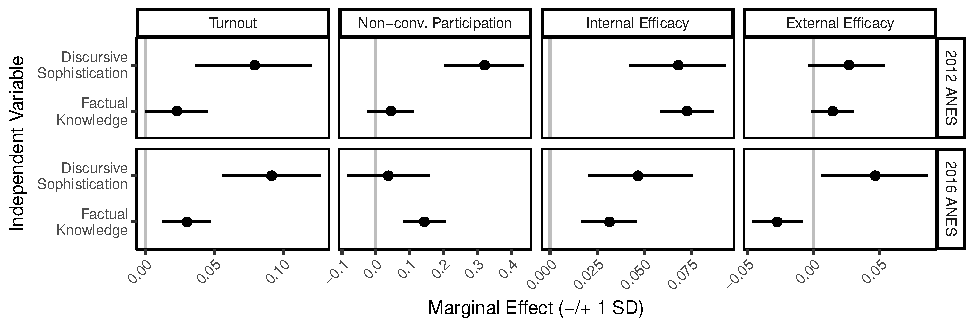
\includegraphics[width=\textwidth]{../fig/knoweff_lwc.pdf}
  \end{figure}
\end{frame}

\subsection{Control for Personality}
\begin{frame}{\hyperlink{engagement}{Engagement and Participation -- Control for Personality}}\label{engagement_personality}
  \begin{figure}
  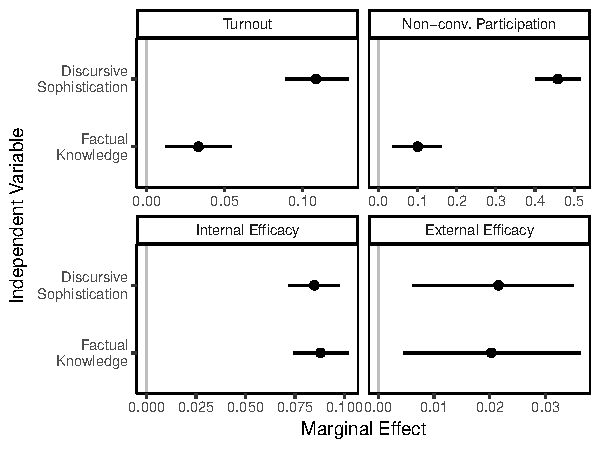
\includegraphics[width=\textwidth]{../fig/knoweff_personality.pdf}
  \end{figure}
\end{frame}

\subsection{Determinants of Sophistication}
\begin{frame}{Determinants of Sophistication}
\begin{figure}
	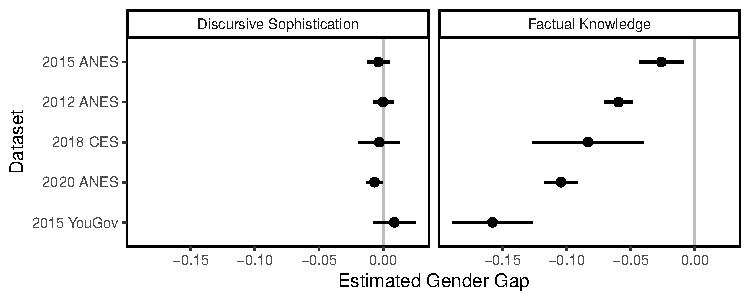
\includegraphics[height=.9\textheight]{../fig/determinants.pdf}
\end{figure}
\end{frame}

%\section{Additional Analyses}
%
%\subsection{Precision in Perceived Ideological Position}
%\begin{frame}{Precision in Perceived Ideological Position (2012 ANES)}\label{hetreg}
%  \begin{figure}
%  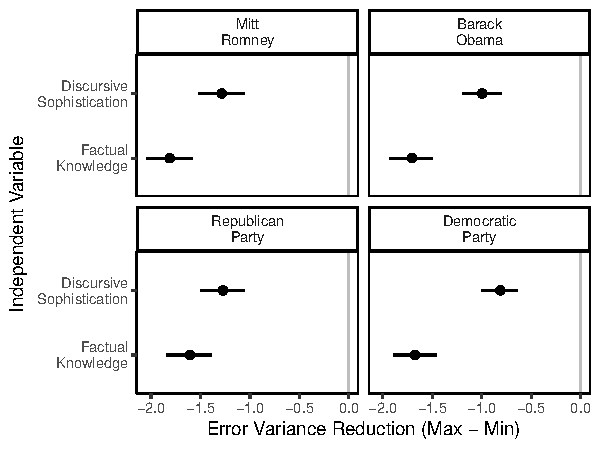
\includegraphics{fig/hetreg_pres.pdf}
%  \end{figure}
%\end{frame}
%
%\subsection{Consistency with Initial Vote Intention}
%\begin{frame}{Consistency with Initial Vote Intention (2012 ANES)}\label{prepost}
%  \begin{figure}
%  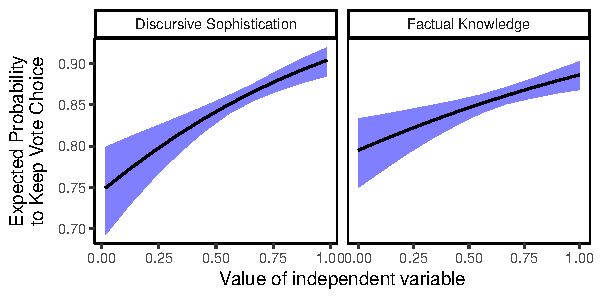
\includegraphics{fig/prepost_exp.pdf}
%  \end{figure}
%\end{frame}
%
%\subsection{Issue-Consistency: Support for Redistribution}
%\begin{frame}{Issue-Consistency: Support for Redistribution (2012 ANES)}\label{redistribution}
%  \begin{figure}
%  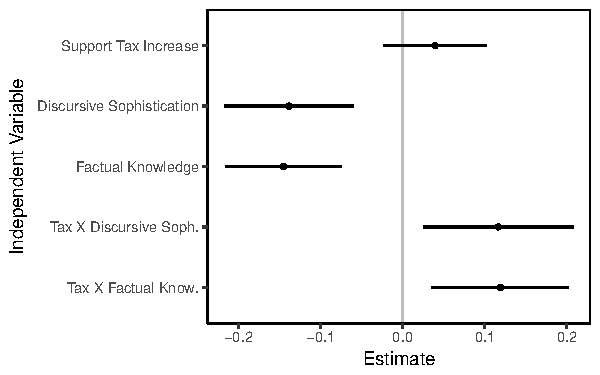
\includegraphics{fig/redistribution.pdf}
%  \end{figure}
%\end{frame}
%% Prior (2014): Visual Political Knowledge

\begin{frame} %<beamer:0> % hide references
  \frametitle{References}
  \def\newblock{\hskip .11em plus .33em minus .07em}
  %\nocite{*}
  \begin{scriptsize}
    \bibliographystyle{/data/Dropbox/Uni/Lit/apsr2006}
    \bibliography{/data/Dropbox/Uni/Lit/Literature}
  \end{scriptsize}
\end{frame}

\end{document}